\documentclass[
  notitle,
  nojss,
  noheadings]{jss}

\usepackage[utf8]{inputenc}

\providecommand{\tightlist}{%
  \setlength{\itemsep}{0pt}\setlength{\parskip}{0pt}}

\author{
Nicolas Bennett\footnotemark[1]\\ETH Zürich \And Drago
Plečko\footnotemark[1]\footnotetext[1]{These authors contributed equally.}\\ETH Zürich \And Ida-Fong Ukor\\Monash Health \AND Nicolai Meinshausen\\ETH Zürich \And Peter Bühlmann\\ETH Zürich
}
\title{\pkg{ricu}: \proglang{R}'s Interface to Intensive Care Data}

\Plainauthor{Nicolas Bennett\footnotemark[1], Drago
Plečko\footnotemark[1]\footnotetext[1]{These authors contributed equally.}, Ida-Fong Ukor, Nicolai Meinshausen, Peter Bühlmann}
\Plaintitle{ricu: R's Interface to Intensive Care Data}
\Shorttitle{\pkg{ricu}: \proglang{R} meets ICU data}

\Abstract{
Providing computational infrastructure for handling diverse intensive
care unit (ICU) datasets, the \proglang{R} package \pkg{ricu} enables
writing dataset-agnostic analysis code, thereby facilitating
multi-center training and validation of machine learning models. The
package is designed with an emphasis on extensibility both to new
datasets as well as clinical data concepts, and currently supports the
loading of around 100 patient variables corresponding to a total of
395,941 ICU admissions from five data sources collected in Europe and
the United States. By allowing for the addition of user-specified
medical concepts and data sources, the aim of \pkg{ricu} is to foster
robust, data-based intensive care research, allowing the user to
externally validate their method or conclusion with relative ease, and
in turn facilitating reproducible and therefore transparent work in this
field.
}

\Keywords{electronic health records, computational physiology, critical care medicine}
\Plainkeywords{electronic health records, computational physiology, critical care medicine}

%% publication information
%% \Volume{50}
%% \Issue{9}
%% \Month{June}
%% \Year{2012}
%% \Submitdate{}
%% \Acceptdate{2012-06-04}

\Address{
    Nicolas Bennett\footnotemark[1]\\
    ETH Zürich\\
    Seminar for Statistics\\
Rämistrasse 101\\
CH-8092 Zurich\\
  E-mail: \email{nicolas.bennett@stat.math.ethz.ch}\\
  
      Drago
  Plečko\footnotemark[1]\footnotetext[1]{These authors contributed equally.}\\
    ETH Zürich\\
    Seminar for Statistics\\
Rämistrasse 101\\
CH-8092 Zürich\\
  E-mail: \email{drago.plecko@stat.math.ethz.ch}\\
  
      Ida-Fong Ukor\\
    Monash Health\\
    Department of Anaesthesiology and Perioperative Medicine\\
246 Clayton Road\\
Clayton VIC 3168\\
  E-mail: \email{ida-fong.ukor@monashhealth.org}\\
  
      Nicolai Meinshausen\\
    ETH Zürich\\
    Seminar for Statistics\\
Rämistrasse 101\\
CH-8092 Zürich\\
  E-mail: \email{meinshausen@stat.math.ethz.ch}\\
  
      Peter Bühlmann\\
    ETH Zürich\\
    Seminar for Statistics\\
Rämistrasse 101\\
CH-8092 Zürich\\
  E-mail: \email{peter.buehlmann@stat.math.ethz.ch}\\
  
  }

% Pandoc citation processing

% Pandoc header

\usepackage{amsmath} \usepackage{booktabs} \usepackage{makecell} \usepackage{threeparttablex} \usepackage{pdflscape}

\begin{document}

\maketitle

\renewcommand*{\thefootnote}{\fnsymbol{footnote}}
\footnotetext{$^{*}$These authors contributed equally.}
\renewcommand*{\thefootnote}{\arabic{footnote}}

\hypertarget{introduction}{%
\section{Introduction}\label{introduction}}

Collection of electronic health records has seen a significant rise in
recent years \citep{evans2016}, opening up opportunities and providing
the grounds for a large body of data-driven research oriented towards
helping clinicians in decision-making and therefore improving patient
care and health outcomes \citep{jiang2017}. While growing amounts of
collected patient data might contribute to an increasingly hard task for
intensivists to focus on relevant subsets thereof \citep{pickering2013},
this poses an opportunity for the application of machine learning (ML)
methods.

One example of a problem that has received much attention from the ML
community is early prediction of sepsis in the intensive care unit
\citep[ICU;][]{desautels2016, nemati2018, futoma2017, kam2017}.
Interestingly, there is evidence that a large proportion of the
publications are based on the same dataset \citep{fleuren2019}, the
Medical Information Mart for Intensive Care III
\citep[MIMIC-III;][]{johnson2016}, which shows a systematic lack of
external validation. This issue has recently again been highlighted by a
study demonstrating poor performance in external validation of a widely
adopted proprietary sepsis prediction model \citep{wong2021}.

Contributing to this problem might well be the lack of computational
infrastructure handling multiple datasets. The MIMIC-III dataset
consists of 26 different tables containing about 20GB of data. While
much work and care has gone into data preprocessing in order to provide
a self-contained ready-to-use data resource with MIMIC-III, seemingly
simple tasks such as computing a Sepsis-3 label \citep{singer2016}
remain non-trivial efforts\footnote{There is considerable heterogeneity
  in number of patients satisfying the Sepsis-3 criterion
  \citep{singer2016} among studies investigating MIMIC-III. Reported
  Sepsis-3 prevalence ranges from 11.3\% \citep{desautels2016}, over
  23.9\% \citep{nemati2018} and 25.4\% \citep{wang2018}, up to 49.1\%
  \citep{johnson2018}. While some of this variation may be explained by
  differing patient inclusion criteria, diversity in label
  implementation must also contribute significantly.}. This is only
exacerbated when aiming to co-integrate multiple different datasets of
this form, spanning hospitals and even countries, in order to capture
effects of differing practice and demographics.

The aim of \pkg{ricu} is to provide computational infrastructure
allowing users to investigate complex research questions in the context
of critical care medicine as easily as possible by providing a unified
interface to a heterogeneous set of data sources. The package enables
users to write dataset-agnostic code which can simplify implementation
and shorten the time necessary for prototyping code querying different
datasets. In its current form, the package handles five large-scale,
publicly available intensive care databases out of the box: MIMIC-III
from the Beth Israel Deaconess Medical Center in Boston, Massachusetts
\citep[BIDMC;][]{johnson2016}, the eICU Collaborative Research Database
\citep{pollard2018}, containing data collected from 208 hospitals across
the United States, the High Time Resolution ICU Dataset (HiRID) from the
Department of Intensive Care Medicine of the Bern University Hospital,
Switzerland \citep{faltys2021}, the Amsterdam University Medical Center
Database (AmsterdamUMCdb) from the Amsterdam University Medical Center
\citep{thoral2021} and MIMIC-IV, again using data from BIDMC
\citep{johnson2021}. Furthermore, \pkg{ricu} was designed with
extensibility in mind such that adding new public and/or private
user-provided datasets is possible. Being implemented in \proglang{R}, a
programming language popular among statisticians and data analysts, it
is our hope to contribute to accessible and reproducible research by
using a familiar environment and requiring only few system dependencies,
thereby simplifying setup considerably.

To our knowledge, infrastructure that provides a common interface to
multiple such datasets is a novel contribution. While there have been
efforts \citep{adibuzzaman2016, wang2020} attempting to abstract away
some specifics of a dataset, these have so far exclusively focused on
MIMIC-III, the most popular of public ICU datsets, and have not been
designed with dataset interoperability in mind.

Given the somewhat narrow focus of the targeted datasets, it may come as
a surprise as to how heterogeneous the resulting datasets are. In
MIMIC-III and HiRID, for example, time-stamps are reported as absolute
times (albeit randomly shifted due to data privacy concerns), whereas
eICU and AmsterdamUMCdb use relative times (with origins being admission
times). Another example involves different types of patient identifiers
and their use among datasets. Common to all is the notion of an ICU
admission identifier (ID), but apart from that, the amount of available
information varies: While ICU (and hospital) readmissions for a given
patient can be identified in some, this is not possible in other
datasets. Furthermore, use of identifier systems might not be consistent
over tables. In MIMIC-III, for example, some tables refer to ICU stay
IDs while others use hospital stay IDs, which slightly complicates data
retrieval for a fixed ID system. Additionally, table layouts vary
(\emph{long} versus \emph{wide} data arrangement) and data organization
in general is far from consistent over datasets.

\hypertarget{quick-start-guide}{%
\section{Quick start guide}\label{quick-start-guide}}

The following list gives a quick outline of the steps required for
setting up and starting to use \pkg{ricu}, alongside some section
references on where to find further details. A more comprehensive
version of this overview is available as a
\href{https://CRAN.R-project.org/package=ricu/vignettes/ricu.html}{separate
vignette}.

\begin{enumerate}
\def\labelenumi{\arabic{enumi}.}
\item
  Package installation:

  \begin{itemize}
  \item
    Installation from \href{https://CRAN.R-project.org}{CRAN} as
    \texttt{install.packages("ricu")} provides the most recently
    released version of \pkg{ricu}.
  \item
    Alternatively, the latest development version is available from
    \href{https://github.com/eth-mds/ricu}{GitHub} by running
    \texttt{remotes::install\_github("eth-mds/ricu")}.
  \end{itemize}
\item
  Requesting access to datasets and data source setup:

  \begin{itemize}
  \item
    Demo datasets can be set up by installing the data packages
    \texttt{mimic.demo} and/or \texttt{eicu.demo} from
    \href{\%22https://eth-mds.github.io/physionet-demo\%22}{GitHub}
    using \texttt{install.packages()} as shown in Section
    \ref{ready-to-use-datasets}.
  \item
    The complete MIMIC-III, eICU, HiRID and MIMIC-IV datasets can be
    accessed by \href{https://physionet.org/register}{registering} and
    setting up a
    \href{https://physionet.org/settings/credentialing}{credentialed
    account} at \href{https://physionet.org}{PhysioNet}.
  \item
    Access to AmsterdamUMCdb can be requested via the
    \href{https://amsterdammedicaldatascience.nl/\#amsterdamumcdb}{Amsterdam
    Medical Data Science Website}.
  \item
    The obtained credentials can be configured for PhysioNet datasets by
    setting environment variables \texttt{RICU\_PHYSIONET\_USER} and
    \texttt{RICU\_PHYSIONET\_PASS}, while the download token for
    AmsterdamUMCdb can be set as \texttt{RICU\_AUMC\_TOKEN}.
  \item
    Datasets are downloaded and set up either automatically upon the
    first access attempt or manually by running
    \texttt{setup\_data\_src()}; the environment variable
    \texttt{RICU\_DATA\_PATH} can be set to control data location.
  \item
    Dataset availability can be queried by calling
    \texttt{src\_data\_avail()}.
  \end{itemize}

  A more detailed description of the supported datasets is given in
  Section \ref{ready-to-use-datasets}, summarized in Table
  \ref{tab:datasets}, while Section \ref{data-sources} provides
  implementation details, elaborating on how datasets are represented in
  code.
\item
  Loading of data corresponding to clinical concepts using
  \texttt{load\_concepts()}:

  \begin{itemize}
  \item
    Currently, over 100 data concepts are available for the 4 supported
    datasets (see
    \texttt{concept\_availability()}/\texttt{explain\_dictionary()} for
    names, availability etc.).
  \item
    For example, glucose and age data can be loaded by passing
    \texttt{c("age",\ "glu")} to \texttt{load\_concepts()}.
  \end{itemize}

  Section \ref{data-concepts} goes into more detail on how data concepts
  are represented within \pkg{ricu} and an overview of the preconfigured
  concepts is available from Section \ref{ready-to-use-concepts}.
\item
  Extending the concept dictionary:

  \begin{itemize}
  \item
    Data concepts can be specified in code using the constructors
    \texttt{concept()}/\texttt{item()} or
    \texttt{new\_concept()}/\texttt{new\_item()}.
  \item
    For session persistence, data concepts can also be specified as JSON
    formatted objects.
  \item
    JSON-based concept dictionaries can either extend or replace others
    and they can be pointed to by setting the environment variable
    \texttt{RICU\_CONFIG\_PATH}.
  \end{itemize}

  The JSON format used to encode data concepts is discussed in more
  detail in Section \ref{concept-specification}.
\item
  Adding new datasets:

  \begin{itemize}
  \item
    A JSON-based dataset configuration file is required, from which the
    configuration objects described in Section
    \ref{data-source-configuration} are created.
  \item
    In order for concepts to be available from the new dataset, the
    dictionary requires extension by adding new data items.
  \end{itemize}

  Further information about adding a new dataset is available from
  Section \ref{adding-external-datasets}. Some code used when
  AmsterdamUMCdb was not yet fully integrated with \pkg{ricu} is
  available from \href{https://github.com/eth-mds/aumc}{GitHub} and is
  used for demonstration purposes to set up AmsterdamUMCdb as an
  external dataset \texttt{aumc\_ext}.
\end{enumerate}

Finally, Section \ref{examples} shows briefly how \pkg{ricu} could be
used in practice to address clinical questions by presenting two small
examples.

\hypertarget{ready-to-use-datasets}{%
\section{Ready-to-use datasets}\label{ready-to-use-datasets}}

Several large-scale ICU datasets collected from multiple hospitals in
the US and Europe can be set up for access using \pkg{ricu} with minimal
user effort. Provisions in terms of required configuration information
alongside functions for download and setup are part of \pkg{ricu},
opening up easy access to these datasets. Data itself, however, is not
part of \pkg{ricu} and while the supported datasets are publicly
available, access has to be granted by the dataset creators
individually. Four datasets, MIMIC-III, MIMIC-IV, eICU and HiRID are
hosted on PhysioNet \citep{goldberger2000}, access to which requires an
\href{https://physionet.org/register/}{account}, while the fifth,
AmsterdamUMCdb is currently distributed via a separate platform,
requiring a
\href{https://amsterdammedicaldatascience.nl/\#amsterdamumcdb}{download
link}.

For both MIMIC-III and eICU, small subsets of data are available as demo
datasets that do not require credentialed access to PhysioNet. As the
terms for distribution of these demo datasets are less restrictive, they
can be made available as data packages \pkg{mimic.demo} and
\pkg{eicu.demo}. Due to size constraints, however they are not available
via CRAN, but can be installed from GitHub as

\begin{CodeChunk}
\begin{CodeInput}
R> install.packages(
+   c("mimic.demo", "eicu.demo"),
+   repos = "https://eth-mds.github.io/physionet-demo"
+ )
\end{CodeInput}
\end{CodeChunk}

Provisions for datasets configured to be attached during package loading
are made irrespective of whether data is actually available. Upon access
of an incomplete dataset, the user is asked for permission to download
in interactive sessions and an error is thrown otherwise. Credentials
can either be provided as environment variables
(\texttt{RICU\_PHYSIONET\_USER} and \texttt{RICU\_PHYSIONET\_PASS} for
access to PhysioNet data, as well as \texttt{RICU\_AUMC\_TOKEN} for
AmsterdamUMCdb) and if the corresponding variables are unset, user input
is again required in interactive sessions. For non-interactive sessions,
functionality is exported such that data can be downloaded and set up
ahead of first access (see \texttt{?setup\_src\_data}).

Contingent on being granted access by the data owners, download requires
a stable Internet connection, as well as 50 to 100 GB of temporary disk
storage for unpacking and preparing the data for efficient access. In
terms of permanent storage, 5 to 10 GB per dataset are required (see
Table \ref{tab:datasets}), while memory requirements are kept reasonably
low by iterating over row-chunks for setup operations. Laptop class
hardware (8-16 GB of memory) should suffice for setup and many analysis
tasks which focus only on subsets of rows (and columns). Initial data
source setup (depending on available download speeds and CPU/disk type)
may take upwards of an hour per dataset.

The following paragraphs serve to give quick introductions to the
included datasets, outlining some strengths and weaknesses of each of
the datasets. Especially the PhysioNet datasets
\href{https://mimic.mit.edu/docs/}{MIMIC-III and MIMIC-IV}, as well as
\href{https://eicu-crd.mit.edu/about/eicu/}{eICU} offer good
documentation on the respective websites. Datasets are listed in order
of being added to \pkg{ricu} and the section is concluded with a table
summarizing similarities and differences among the datasets (see Table
\ref{tab:datasets}).

\hypertarget{mimic-iii}{%
\subsection{MIMIC-III}\label{mimic-iii}}

The \href{https://physionet.org/content/mimiciii/1.4/}{Medical
Information Mart for Intensive Care III (MIMIC-III)} represents the
third iteration of the arguably most influential initiative for
collecting and providing large-scale ICU data to the public\footnote{The
  initial MIMIC (at the time short for Multi-parameter Intelligent
  Monitoring for Intensive Care) data release dates back 20 years and
  initially contained data on roughly 100 patients recorded from patient
  monitors in the medical, surgical, and cardiac intensive care units of
  Boston's Beth Israel Hospital during the years 1992-1999
  \citep{moody1996}. Significantly broadened in scope, MIMIC-II was
  released 10 years after, now including data on almost 27,000 adult
  hospital admissions collected from ICUs of Beth Israel Deaconess
  Medical Center from 2001 to 2008 \citep{lee2011}.}. The dataset
comprises de-identified health related data of roughly 46,000 patients
admitted to critical care units of BIDMC during the years 2001-2012.
Amounting to just over 61,000 individual ICU admission, data is
available on demographics, routine vital sign measurements (at
approximately 1 hour resolution), laboratory tests, medication, as well
as critical care procedures, organized as a 26-table relational
structure.

\begin{CodeChunk}
\begin{CodeInput}
R> mimic
\end{CodeInput}
\begin{CodeOutput}
<mimic_env[26]>
        admissions            callout         caregivers        chartevents 
     [58,976 x 19]      [34,499 x 24]        [7,567 x 4] [330,712,483 x 15] 
         cptevents              d_cpt    d_icd_diagnoses   d_icd_procedures 
    [573,146 x 12]          [134 x 9]       [14,567 x 4]        [3,882 x 4] 
           d_items         d_labitems     datetimeevents      diagnoses_icd 
     [12,487 x 10]          [753 x 6]   [4,485,937 x 14]      [651,047 x 5] 
          drgcodes           icustays     inputevents_cv     inputevents_mv 
     [125,557 x 8]      [61,532 x 12]  [17,527,935 x 22]   [3,618,991 x 31] 
         labevents microbiologyevents         noteevents       outputevents 
  [27,854,055 x 9]     [631,726 x 16]   [2,083,180 x 11]   [4,349,218 x 13] 
          patients      prescriptions procedureevents_mv     procedures_icd 
      [46,520 x 8]   [4,156,450 x 19]     [258,066 x 25]      [240,095 x 5] 
          services          transfers 
      [73,343 x 6]     [261,897 x 13] 
\end{CodeOutput}
\end{CodeChunk}

One thing of note from a data-organizational perspective is that a
change in electronic health care systems occurred in 2008. Owing to
this, roughly 38,000 ICU admissions spanning the years 2001 though 2008
are documented using the CareVue system, while for 2008 and onwards,
data was extracted from the MetaVision clinical information system. Item
identifiers differ between the two systems, requiring queries to
consider both ID mappings (heart rate for example being available both
as \texttt{itemid} number \texttt{211} for CareVue and \texttt{220045}
for MetaVision) as does documentation of infusions and other procedures
that are considered as input events (cf., \texttt{inputevents\_cv} and
\texttt{inputevents\_mv} tables). Especially with respect to such input
event data, MetaVision generally provides data of superior quality.

In terms of patient identifiers, MIMIC-III allows for identifying both
individual patients (\texttt{subject\_id}) across hospital admissions
(\texttt{hadm\_id}) and for connecting ICU (re)admissions
(\texttt{icustay\_id}) to hospital admissions. Using the respective
one-to-many relationships, \pkg{ricu} can retrieve patient data using
any of the above IDs, irrespective of how the raw data is organized.

\hypertarget{eicu}{%
\subsection{eICU}\label{eicu}}

Unlike the single-center focus of other datasets, the
\href{https://physionet.org/content/eicu-crd/2.0/}{eICU Collaborative
Research Database} constitutes an amalgamation of data from critical
care units of over 200 hospitals throughout the continental United
States. Large-scale data collected via the Philips eICU program, which
provides telehealth infrastructure for intensive care units, is
available from the Philips eICU Research Institute (eRI), albeit neither
publicly nor freely. Only data corresponding to roughly 200,000 ICU
admissions, sampled from a larger population of over 3 million ICU
admissions and stratified by hospital, is being made available via
PhysioNet. Patients with discharge dates in 2014 or 2015 were
considered, with stays in low acuity units being removed.

\begin{CodeChunk}
\begin{CodeInput}
R> eicu
\end{CodeInput}
\begin{CodeOutput}
<eicu_env[31]>
            admissiondrug               admissiondx                   allergy 
           [874,920 x 14]             [626,858 x 6]            [251,949 x 13] 
             apacheapsvar       apachepatientresult             apachepredvar 
           [171,177 x 26]            [297,064 x 23]            [171,177 x 51] 
     careplancareprovider               careplaneol           careplangeneral 
            [502,765 x 8]               [1,433 x 5]           [3,115,018 x 6] 
             careplangoal careplaninfectiousdisease                 customlab 
            [504,139 x 7]               [8,056 x 8]               [1,082 x 7] 
                diagnosis                  hospital              infusiondrug 
          [2,710,672 x 7]                 [208 x 4]           [4,803,719 x 9] 
             intakeoutput                       lab                medication 
        [12,030,289 x 12]         [39,132,531 x 10]          [7,301,853 x 15] 
                 microlab                      note           nurseassessment 
             [16,996 x 7]           [2,254,179 x 8]          [15,602,498 x 8] 
                nursecare             nursecharting               pasthistory 
          [8,311,132 x 8]         [151,604,232 x 8]           [1,149,180 x 8] 
                  patient              physicalexam           respiratorycare 
           [200,859 x 29]           [9,212,316 x 6]            [865,381 x 34] 
      respiratorycharting                 treatment            vitalaperiodic 
         [20,168,176 x 7]           [3,688,745 x 5]         [25,075,074 x 13] 
            vitalperiodic 
       [146,671,642 x 19] 
\end{CodeOutput}
\end{CodeChunk}

The data is organized into 31 tables and includes patient demographics,
routine vital signs, laboratory measurements, medication
administrations, admission diagnoses, as well as treatment information.
Owing to the wide range of hospitals participating in this data
collection initiative, spanning small, rural, non-teaching health
centers with fewer than 100 beds to large teaching hospitals with an
excess of 500 beds, data availability varies. Even if data was being
recorded at the bedside it might end up missing from the eICU dataset
due to technical limitations of the collection process. As for patient
identifiers, while it is possible to link ICU admissions corresponding
to the same hospital stay, it is not possible to identify patients
across hospital stays.

Data resolution again varies considerably over included variables. The
\texttt{vitalperiodic} table stands out as one of the few examples of a
\emph{wide} table organization (laying out variables as columns), as
opposed to the \emph{long} presentation (following an
entity--attribute--value model) of most other tables containing patient
measurement data. The average time step in \texttt{vitalperiodic} is
around 5 minutes, but data missingness ranges from around 1\% for heart
rate and pulse oximetry to roughly 10\% for respiration rate and up to
80\% for systemic and 90\% for pulmonary artery blood pressure
measurements, therefore giving approximately hourly resolution for such
variables.

\hypertarget{hirid}{%
\subsection{HiRID}\label{hirid}}

Developed for early prediction of circulatory failure
\citep{hyland2020}, the
\href{https://physionet.org/content/hirid/1.0/}{High Time Resolution ICU
Dataset (HiRID)} contains data on almost 34,000 admissions to the
Department of Intensive Care Medicine of the Bern University Hospital,
Switzerland, an interdisciplinary 60-bed unit. Given the clear focus on
a concrete application during data collection, this dataset is the most
limited in terms of data breadth, which is also reflected in a
comparatively simple data layout comprising only 5 tables\footnote{The
  data is available in three states: as raw data and in two intermediary
  preprocessing stages explained in \cite{hyland2020}. While \pkg{ricu}
  focuses exclusively on raw data, the \emph{merged} stage represents a
  selection of variables that were deemed most predictive for
  determining circulatory failure, which are then merged into 18
  meta-variables, representing different clinical concepts. Time stamps
  in \emph{merged} data are left unchanged, yielding irregular time
  series, whereas for the \emph{imputed} stage, data is down-sampled to
  a 5 minute grid and missing values are imputed using a scheme
  discussed in \cite{hyland2020}.}.

\begin{CodeChunk}
\begin{CodeInput}
R> hirid
\end{CodeInput}
\begin{CodeOutput}
<hirid_env[5]>
          general      observations           ordinal            pharma 
     [33,905 x 5] [776,921,131 x 8]          [72 x 3] [16,270,399 x 14] 
        variables 
        [712 x 5] 
\end{CodeOutput}
\end{CodeChunk}

Collected during the period of January 2008 through June 2016, roughly
700 distinct variables covering routine vital signs, diagnostic test
results and treatment parameters are available with variables monitored
at the bedside being recorded with two minute time resolution. In terms
of demographic information and patient identifier systems however, the
data is limited. It is not possible to identify subsequent ICU
admissions corresponding to the same patient and apart from patient age,
sex, weight and height, very little information is available to
characterize patients. There is no medical history, no admission
diagnoses, only in-ICU mortality information, no unstructured patient
data and no information on patient discharge. Furthermore, data on body
fluid sampling has been omitted, complicating for example the
construction of a Sepsis-3 label \citep{singer2016}.

\hypertarget{amsterdamumcdb}{%
\subsection{AmsterdamUMCdb}\label{amsterdamumcdb}}

As a second European dataset, also focusing on increased time-resolution
over the US datasets,
\href{https://amsterdammedicaldatascience.nl/\#amsterdamumcdb}{AmsterdamUMCdb}
has been made available in late 2019, containing data on over 23,000
intensive care unit and high dependency unit admissions of adult
patients during the years 2003 through 2016. The department of Intensive
Care at Amsterdam University Medical Center is a mixed medical-surgical
ICU with 32 bed intensive care and 12 bed high dependency units with an
average of 1000-2000 yearly admissions. Covering middle ground between
the US datasets and HiRID in terms of breadth of included data, while
providing a maximal time-resolution of 1 minute, AmsterdamUMCdb
constitutes a well organized high quality ICU data resource organized
succinctly as a 7-table relational structure.

\begin{CodeChunk}
\begin{CodeInput}
R> aumc
\end{CodeInput}
\begin{CodeOutput}
<aumc_env[7]>
         admissions           drugitems       freetextitems 
      [23,106 x 17]    [4,907,269 x 31]      [651,248 x 11] 
          listitems        numericitems procedureorderitems 
  [30,744,065 x 11]  [977,625,612 x 15]     [2,188,626 x 8] 
       processitems 
      [256,715 x 6] 
\end{CodeOutput}
\end{CodeChunk}

For data anonymization purposes, demographic information such as patient
weight, height and age only available as binned variables instead of raw
numeric values. Apart from this, there is information on patient origin,
mortality, admission diagnoses, as well as numerical measurements
including vital parameters, lab results, outputs from drains and
catheters, information on administered medication, and other medical
procedures. In terms of patient identifiers, it is possible to link ICU
admissions corresponding to the same individual, but it is not possible
to identify separate hospital admissions.

\hypertarget{mimic-iv}{%
\subsection{MIMIC-IV}\label{mimic-iv}}

The most recently released dataset and next iteration in the MIMIC line
of datasets, MIMIC-IV, has recently been released as first stable
version \citep{johnson2021} and support in \pkg{ricu} is available as
dataset \texttt{miiv}. Compared to MIMIC-III, this release shifts focus
to newer data, dropping all CareVue-documented patients and with that,
patients who were admitted before 2008, while adding patients admitted
up to and including 2019. The resulting dataset contains data on over
256,000 patients of which, 53,000 were admitted to ICUs, resulting in
76,000 unique ICU and almost 70,000 related hospital admissions.

\begin{CodeChunk}
\begin{CodeInput}
R> miiv
\end{CodeInput}
\begin{CodeOutput}
<miiv_env[27]>
        admissions        chartevents            d_hcpcs    d_icd_diagnoses 
    [523,740 x 15] [329,499,788 x 10]       [89,200 x 4]      [109,775 x 3] 
  d_icd_procedures            d_items         d_labitems     datetimeevents 
      [85,257 x 3]        [3,861 x 9]        [1,630 x 5]    [7,495,712 x 9] 
     diagnoses_icd           drgcodes               emar        emar_detail 
   [5,280,351 x 5]      [769,622 x 7]  [27,464,367 x 11]  [55,947,921 x 33] 
       hcpcsevents           icustays        inputevents          labevents 
     [160,727 x 6]       [76,540 x 8]   [9,460,658 x 26] [122,103,667 x 15] 
microbiologyevents       outputevents           patients           pharmacy 
  [3,397,914 x 24]    [4,457,381 x 8]      [382,278 x 6]  [14,736,386 x 27] 
               poe         poe_detail      prescriptions    procedureevents 
 [42,483,962 x 11]    [3,256,358 x 5]  [17,008,053 x 17]     [731,247 x 26] 
    procedures_icd           services          transfers 
     [779,625 x 6]      [562,892 x 5]    [2,189,535 x 7] 
\end{CodeOutput}
\end{CodeChunk}

\begin{table}

\caption{\label{tab:datasets}Comparison of datasets supported by \pkg{ricu}, highlighting some of the major similarities and distinguishing features among the five data sources described in the preceding sections. Values followed by parenthesized ranges represent medians and are accompanied by interquartile ranges.}
\centering
\begin{threeparttable}
\begin{tabular}[t]{lll}
\toprule
  & MIMIC (demo) & eICU (demo)\\
\midrule
Number of tables & 25 & 31\\
Disk storage [GB] & 0.01 & 0.06\\
Largest table [rows] & 758,355 & 1,634,960\\
Available concepts\textsuperscript{*} & 89 & 86\\
\addlinespace[0.3em]
\multicolumn{3}{l}{\textbf{Data collection}}\\
\hspace{1em}Time span & NA & NA\\
\hspace{1em}Country of origin & NA & NA\\
\addlinespace[0.3em]
\multicolumn{3}{l}{\textbf{Admission counts}}\\
\hspace{1em}ICU & 136 & 2,520\\
\hspace{1em}Hospital & 129 & 2,174\\
\hspace{1em}Unique patients & 100 & -\\
\addlinespace[0.3em]
\multicolumn{3}{l}{\textbf{Stay lengths [day]}}\\
\hspace{1em}ICU stays & 2.11 (1.23--4.33) & 1.47 (0.79--2.78)\\
\hspace{1em}Hospital stays & 6.63 (3.31--10.65) & 4.14 (2.12--7.90)\\
\addlinespace[0.3em]
\multicolumn{3}{l}{\textbf{Vital signs [1/hour]}}\\
\hspace{1em}Heart rate & 1.00 (1.00--1.00) & 12.00 (12.00--12.00)\\
\hspace{1em}Mean arterial pressure & 1.00 (1.00--1.00) & 12.00 (4.00--12.00)\\
\addlinespace[0.3em]
\multicolumn{3}{l}{\textbf{Lab tests [1/day]}}\\
\hspace{1em}Bilirubin & 1.02 (0.98--2.01) & 1.00 (0.89--1.16)\\
\hspace{1em}Lactate & 5.00 (1.75--10.75) & 3.69 (1.38--6.40)\\
\bottomrule
\end{tabular}
\begin{tablenotes}
\item[*] These values represent the number of atomic concepts per data source. Additionally, 28 recursive concepts are available, which build on data source specific atomic concepts in a source agnostic manner (see Section \ref{concept-specification} for details).
\end{tablenotes}
\end{threeparttable}
\end{table}

\begin{quote}
Note: The following code blocks are run using demo (\texttt{mimic\_demo}
and \texttt{eicu\_demo}) instead of full (\texttt{mimic\_demo} and
\texttt{eicu\_demo}) datasets and therefore might be less useful. For
data set up, please consult the manual at \texttt{?attach\_src}. The
full version of this vignette is available from
\href{https://CRAN.R-project.org/package=ricu/vignettes/jss.pdf}{CRAN}.
\end{quote}

In addition to including newer ICU data, this MIMIC release puts both
more emphasis on data collected outside the ICU, newly making emergency
department (ED) data available. In a similar vein, the set of considered
data types is also expanded by including chest X-ray (CXR) imagery
directly with MIMIC data, using the same patient identifiers, while
expanding the amount of unstructured text data (still to be made
publicly available). Despite these promising developments, the focus of
\pkg{ricu} remains on data that lies in the intersection of the
supported datasets and therefore both ED and CXR data cannot be accessed
by the current \texttt{miiv} implementation. Finally, documentation of
medication administration has been much improved by not only reporting
prescriptions, but, using an electronic Medicine Administration Record
(eMAR) system, including time-stamped data on administration of
individual formulary units.

\hypertarget{data-concepts}{%
\section{Data concepts}\label{data-concepts}}

One of the key components of \pkg{ricu} is a scheme for specifying how
to retrieve data corresponding to predefined clinical concepts from a
given data source. This abstraction provides a mechanism for hiding away
the data source specific implementation of a concept, in turn enabling
dataset agnostic code for analysis. Heart rate, for example can be
loaded from datasets \texttt{mimic\_demo} and \texttt{eicu\_demo} using
the \texttt{hr} concept as

\begin{CodeChunk}
\begin{CodeInput}
R> src  <- "mimic_demo"
R> demo <- c(src, "eicu_demo")
R> 
R> load_concepts("hr", demo, verbose = FALSE)
\end{CodeInput}
\begin{CodeOutput}
# A `ts_tbl`: 152,197 x 4
# Id vars:    `source`, `icustay_id`
# Units:      `hr` [bpm]
# Index var:  `charttime` (1 hours)
        source     icustay_id charttime    hr
        <chr>           <int> <drtn>    <dbl>
      1 eicu_demo      141764   0 hours   119
      2 eicu_demo      141764   1 hours   105
      3 eicu_demo      141764   2 hours    95
      4 eicu_demo      141764   3 hours   106
      5 eicu_demo      141764   4 hours   102
    ...
152,193 mimic_demo     298685 314 hours    60
152,194 mimic_demo     298685 315 hours    56
152,195 mimic_demo     298685 316 hours    50
152,196 mimic_demo     298685 317 hours    48
152,197 mimic_demo     298685 318 hours     0
# ... with 152,187 more rows
\end{CodeOutput}
\end{CodeChunk}

This requires infrastructure for specifying how to retrieve data subsets
(Section \ref{concept-specification}) that is both extensible (to new
concepts and new datasets) and flexible enough to handle
concept-specific preprocessing. Furthermore, allowing for code re-use
for common data transformation tasks is important for simplifying both
code development and maintenance. Building on this framework, \pkg{ricu}
has included a dictionary with over 100 concepts implemented for all
five supported datasets (where possible; see also Section
\ref{ready-to-use-concepts} for further details).

\hypertarget{data-classes}{%
\subsection{Data classes}\label{data-classes}}

In order to represent tabular ICU data, \pkg{ricu} provides several
classes, all inheriting from \texttt{data.table}. The most basic of
which, \texttt{id\_tbl}, marks one (or several) columns as
\texttt{id\_vars} which serve to define a grouping (i.e., identify
patients or unit stays). Inheriting from \texttt{id\_tbl},
\texttt{ts\_tbl} is capable of representing grouped time series data. In
addition to \texttt{id\_var} column(s), a single column is marked as
\texttt{index\_var} and is required to hold a base \proglang{R}
\texttt{difftime} vector. Furthermore, \texttt{ts\_tbl} contains a
scalar-valued \texttt{difftime} object as \texttt{interval} attribute,
specifying the time series step size. More recently, a further class,
\texttt{win\_tbl}, inheriting from \texttt{ts\_tbl} has been added.
Objects of this class can be used for time-stamped measurements
associated with a validity period. A set of drug infusions, consisting
of both rates and intervals can as such be conveniently represented by a
\texttt{win\_tbl} object.

Metadata for classes inheriting from \texttt{id\_tbl} is transiently
added to \texttt{data.table} objects and for S3 generic functions which
allow for object modifications, down-casting is implicit:

\begin{CodeChunk}
\begin{CodeInput}
R> (dat <- ts_tbl(a = 1:5, b = hours(1:5), c = rnorm(5)))
\end{CodeInput}
\begin{CodeOutput}
# A `ts_tbl`: 5 x 3
# Id var:     `a`
# Index var:  `b` (1 hours)
      a b             c
  <int> <drtn>    <dbl>
1     1 1 hours -1.53
2     2 2 hours  1.12
3     3 3 hours -0.0745
4     4 4 hours -0.974
5     5 5 hours  1.98
\end{CodeOutput}
\begin{CodeInput}
R> dat[["b"]] <- dat[["b"]] + mins(30)
R> dat
\end{CodeInput}
\begin{CodeOutput}
# An `id_tbl`: 5 x 3
# Id var:      `a`
      a b                c
  <int> <drtn>       <dbl>
1     1  5400 secs -1.53
2     2  9000 secs  1.12
3     3 12600 secs -0.0745
4     4 16200 secs -0.974
5     5 19800 secs  1.98
\end{CodeOutput}
\end{CodeChunk}

Due to time series step size of \texttt{dat} being specified as 1 hour,
an internal inconsistency is encountered when shifting time stamps by 30
minutes, as time steps are no longer multiples of the time series
interval, in turn causing down-casting to \texttt{id\_tbl}. Furthermore,
if column \texttt{a} were to be removed, direct down-casting to
\texttt{data.table} would be required in order to resolve resulting
inconsistencies\footnote{Updating an object inheriting from
  \texttt{id\_tbl} using \texttt{data.table::set()} bypasses consistency
  checks as this is not an S3 generic function and therefore its
  behavior cannot be tailored to requirements of \texttt{id\_tbl}
  objects. It therefore is up to the user to avoid creating invalid
  \texttt{id\_tbl} objects in such a way.}.

Coercion to base classes \texttt{data.frame} and \texttt{data.table}, by
stripping away the extra attributes, is easily possible using functions
\texttt{as.data.frame()} and \texttt{as.data.table()}. Coercion is also
available as \texttt{data.table}-style by-reference operation by passing
\texttt{by\_ref\ =\ TRUE} to any of the above coercion functions. User
caution is advised, as this does break with base \proglang{R} by-value
(or copy-on-modify) semantics and may lead to unexpected behavior.

In its current form, \texttt{win\_tbl} objects can both be used to
represent for example drug rates or drug amounts, administered over a
specified time-period. When calling the utility function
\texttt{expand()} however, which creates a \texttt{ts\_tbl} from a
\texttt{win\_tbl} by assigning values to the corresponding time steps,
values are assumed to be \emph{valid} for the given interval.

\begin{CodeChunk}
\begin{CodeInput}
R> (dat <- win_tbl(a = 1:5, b = hours(1:5), c = mins(rep(90, 5)),
+                 d = runif(5)))
\end{CodeInput}
\begin{CodeOutput}
# A `win_tbl`:  5 x 4
# Id var:       `a`
# Index var:    `b` (1 hours)
# Duration var: `c`
      a b       c           d
  <int> <drtn>  <drtn>  <dbl>
1     1 1 hours 90 mins 0.124
2     2 2 hours 90 mins 0.430
3     3 3 hours 90 mins 0.237
4     4 4 hours 90 mins 0.735
5     5 5 hours 90 mins 0.135
\end{CodeOutput}
\begin{CodeInput}
R> expand(dat)
\end{CodeInput}
\begin{CodeOutput}
# A `ts_tbl`: 10 x 3
# Id var:     `a`
# Index var:  `b` (1 hours)
       a b           d
   <int> <drtn>  <dbl>
 1     1 1 hours 0.124
 2     1 2 hours 0.124
 3     2 2 hours 0.430
 4     2 3 hours 0.430
 5     3 3 hours 0.237
 6     3 4 hours 0.237
 7     4 4 hours 0.735
 8     4 5 hours 0.735
 9     5 5 hours 0.135
10     5 6 hours 0.135
\end{CodeOutput}
\end{CodeChunk}

In a case where \texttt{d} represented drug amounts instead of drug
rates, the current implementation of \texttt{expand()} would produce
incorrect results. One would expect the overall amount in such a
scenario to be evenly divided by -- and the resulting fractions assigned
to -- the corresponding time steps. Allowing for this distinction is
being considered, but, as of yet, has not been implemented.

Utilizing the attached metadata of objects inheriting from
\texttt{id\_tbl}, several utility functions can be called with concise
semantics (as seen in the above example, where \texttt{expand()} is able
to determine the required column names from the \texttt{win\_tbl} object
by default). Utilities include functions for sorting, checking for
duplicates, aggregating data per combination of \texttt{id\_vars} (and
time step/time duration), checking time series data for gaps, verifying
time series regularity and converting between irregular and regular time
series, as well as functions for several types of moving window
operations. Adding to those class-specific implementations,
\texttt{id\_tbl} objects inherit from \texttt{data.table} (and therefore
from \texttt{data.frame}), ensuring compatibility with a wide range of
functionality targeted at these base-classes.

\hypertarget{ready-to-use-concepts}{%
\subsection{Ready-to-use concepts}\label{ready-to-use-concepts}}

The current selection of clinical concepts that is included with
\pkg{ricu} covers many physiological variables that are available
throughout the included datasets. Treatment-related information on the
other hand, being more heterogeneous in nature and therefore harder to
harmonize across datasets, has been added on an as-needed basis and
therefore is more limited in breadth. A quick note on loading from
multiple sources simultaneously: In the introductory example, heart rate
was loaded from multiple data sources, resulting in a column
\texttt{source} being added. This allows for identifying patient IDs
corresponding to the respective data sources and the extra column is
added to the set of \texttt{id\_vars}. In the following calls to
\texttt{load\_concepts()}, only data from a single source is requested
and therefore no corresponding \texttt{source} column is added.

Available concepts can be enumerated using \texttt{load\_dictionary()}
and the utility function \texttt{explain\_dictionary()} can be used to
display some concept metadata.

\begin{CodeChunk}
\begin{CodeInput}
R> dict <- load_dictionary(demo)
R> head(dict)
\end{CodeInput}
\begin{CodeOutput}
<concept[6]>
                                  abx                              adh_rate 
           antibiotics <lgl_cncpt[4]>       vasopressin rate <num_cncpt[3]> 
                                  adm                                   age 
patient admission type <fct_cncpt[2]>            patient age <num_cncpt[2]> 
                                  alb                                   alp 
               albumin <num_cncpt[2]>   alkaline phosphatase <num_cncpt[2]> 
\end{CodeOutput}
\begin{CodeInput}
R> explain_dictionary(head(dict))
\end{CodeInput}
\begin{CodeOutput}
      name     category            description
1      abx  medications            antibiotics
2 adh_rate  medications       vasopressin rate
3      adm demographics patient admission type
4      age demographics            patient age
5      alb    chemistry                albumin
6      alp    chemistry   alkaline phosphatase
\end{CodeOutput}
\end{CodeChunk}

The following subsections serve to introduce some of the included
concepts as well as highlight limitations that come with current
implementations. Grouping the available concepts by category yields the
following counts

\begin{CodeChunk}
\begin{CodeInput}
R> table(vapply(dict, `[[`, character(1L), "category"))
\end{CodeInput}
\begin{CodeOutput}

   blood gas    chemistry demographics   hematology  medications 
          10           21            6           20           17 
microbiology neurological      outcome       output  respiratory 
           1            8           19            2            9 
      vitals 
           6 
\end{CodeOutput}
\end{CodeChunk}

\hypertarget{physiological-data}{%
\subsubsection{Physiological data}\label{physiological-data}}

The largest and most well established group of concepts (covering more
than half of all currently included concepts) includes physiological
patient measurements such as routine vital signs, respiratory variables,
fluid discharge amounts, as well as many kinds of laboratory tests
including blood gas measurements, chemical analysis of body fluids and
hematology assays.

\begin{CodeChunk}
\begin{CodeInput}
R> load_concepts(c("alb", "glu"), src, interval = mins(15L),
+               verbose = FALSE)
\end{CodeInput}
\begin{CodeOutput}
# A `ts_tbl`: 1,965 x 4
# Id var:     `icustay_id`
# Units:      `alb` [g/dL], `glu` [mg/dL]
# Index var:  `charttime` (15 mins)
      icustay_id charttime    alb   glu
           <int> <drtn>     <dbl> <dbl>
    1     201006 -3495 mins  NA     116
    2     201006 -2745 mins  NA      83
    3     201006 -1275 mins  NA      91
    4     201006    15 mins   2.4   175
    5     201006   675 mins  NA     129
  ...
1,961     298685 15600 mins  NA     159
1,962     298685 16365 mins   2.2   153
1,963     298685 17400 mins  NA     182
1,964     298685 17595 mins  NA     122
1,965     298685 17955 mins   2.5   121
# ... with 1,955 more rows
\end{CodeOutput}
\end{CodeChunk}

Most concepts of this kind are represented by \texttt{num\_cncpt}
objects (see Section \ref{concept-specification}) with an associated
unit of measurement and a range of permissible values. Data is mainly
returned as \texttt{ts\_tbl} objects, representing time-dependent
observations. Apart from conversion to a common unit (using
functionality offered by the \pkg{units} package \citep{pebesma2016} or
possibly using the \texttt{convert\_unit()} callback function), little
has to be done in terms of preprocessing: values are simply reported at
time-points rounded to the requested interval.

\hypertarget{patient-demographics}{%
\subsubsection{Patient demographics}\label{patient-demographics}}

Moving on from dynamic, time-varying patient data, this group of
concepts focuses on static patient information. While the assumption of
remaining constant throughout a stay is likely to hold for variables
including patient sex or height this is only approximately true for
others such as weight. Nevertheless, such effects are ignored and
concepts of this group will be mainly returned as \texttt{id\_tbl}
objects with no corresponding time-stamps included.

Whenever requesting concepts which are returned with associated
time-stamps (e.g., glucose) alongside time-constant data (e.g., age),
merging will duplicate static data over all time-points.

\begin{CodeChunk}
\begin{CodeInput}
R> load_concepts(c("age", "glu"), src, verbose = FALSE)
\end{CodeInput}
\begin{CodeOutput}
# A `ts_tbl`: 1,914 x 4
# Id var:     `icustay_id`
# Units:      `age` [years], `glu` [mg/dL]
# Index var:  `charttime` (1 hours)
      icustay_id charttime   age   glu
           <int> <drtn>    <dbl> <dbl>
    1     201006 -58 hours  68.9   116
    2     201006 -45 hours  68.9    83
    3     201006 -21 hours  68.9    91
    4     201006   0 hours  68.9   175
    5     201006  11 hours  68.9   129
  ...
1,910     298685 260 hours  80.1   159
1,911     298685 272 hours  80.1   153
1,912     298685 290 hours  80.1   182
1,913     298685 293 hours  80.1   122
1,914     298685 299 hours  80.1   121
# ... with 1,904 more rows
\end{CodeOutput}
\end{CodeChunk}

Despite a best-effort approach, data availability can be a limiting
factor. While for physiological variables, there is good agreement even
across countries, data-privacy considerations, as well as lack of a
common standard for data encoding, may cause issues that are hard to
resolve. In some cases, this can be somewhat mitigated while in others,
this is a limitation to be kept in mind. In AmsterdamUMCdb, for example,
patient age, height and weight are not available as continuous
variables, but as factor variables with patients binned into groups.
Such variables are then approximated by returning the respective
mid-points of groups for \texttt{aumc} data\footnote{Prioritizing
  consistency over accuracy, one could apply the same binning to
  datasets which report numeric values, but the concepts included with
  \pkg{ricu} attempt to strike a balance between consistency and amount
  of applied preprocessing. With the extensible architecture of data
  concepts, however, such categorical variants of patient demographic
  concepts could easily be added.}. Other concepts, such as \texttt{adm}
(categorizing admission types) or a potential \texttt{icd} concept
(diagnoses as ICD-9 codes) can only return data if available from the
data source in question. Unfortunately, neither \texttt{aumc} nor
\texttt{hirid} contain ICD-9 encoded diagnoses, and in the case of
\texttt{hirid}, no diagnosis information is available at all.

\hypertarget{treatment-related-information}{%
\subsubsection{Treatment-related
information}\label{treatment-related-information}}

The largest group of concepts dealing with treatment-related information
is described by the \texttt{medications} category. In addition to drug
administrations, only basic ventilation information is currently
provided as ready-to-use concept. Just like availability of common ICU
procedures, patient medication is also underdeveloped, covering mainly
vasopressor administrations, as well as corticosteroids, antibiotics and
dextrose infusions. The current concepts retrieving treatment-related
information are mostly focused on providing data required for
constructing clinical scores described in Section \ref{outcomes}. While
this group of concepts lends itself to use of \texttt{win\_tbl} objects,
a call to \texttt{load\_concepts()}, requesting multiple concepts which
do not all return data as \texttt{win\_tbl} (while leaving the
\texttt{merge} argument at default value \texttt{TRUE}), all
\texttt{win\_tbl} objects are converted to \texttt{ts\_tbl} in order to
be merged with the non-\texttt{win\_tbl} objects.

Ventilation is represented by several concepts: a ventilation indicator
variable (\texttt{vent\_ind}), represented by a \texttt{win\_tbl} object
is constructed from start and end events (concepts \texttt{vent\_start}
and \texttt{vent\_end}). This includes any kind of mechanical
ventilation (invasive via an endotracheal or tracheostomy tube), as well
as non-invasive ventilation via face or nasal masks. In line with other
concepts belonging to this group, the current state is far from being
comprehensive and expansion to further ventilation parameters is
desirable.

The singular concept addressing antibiotics (\texttt{abx}) returns an
indicator signaling whenever an antibiotic was administered. This
includes any route of administration (intravenous, oral, topical, etc.)
and does neither report dosage, nor active ingredient. Finally,
vasopressor administration is reported by several concepts representing
different vasoactive drugs (including dopamine, dobutamine, epinephrine,
norepinephrine and vasopressin), as well as different administration
aspects such as rate, duration and rate administered for at least 60
minutes, which is used in Sepsis-Related Organ Failure Assessment (SOFA)
scoring \citep{vincent1996}.

\begin{CodeChunk}
\begin{CodeInput}
R> load_concepts(c("abx", "vent_ind", "norepi_rate", "norepi_dur"), src,
+               verbose = FALSE)
\end{CodeInput}
\begin{CodeOutput}
# A `ts_tbl`: 12,434 x 6
# Id var:     `icustay_id`
# Units:      `norepi_rate` [mcg/kg/min]
# Index var:  `startdate` (1 hours)
       icustay_id startdate abx   vent_ind norepi_rate norepi_dur
            <int> <drtn>    <lgl> <lgl>          <dbl> <drtn>
     1     201006   7 hours TRUE  NA           NA      NA hours
     2     201006   8 hours NA    TRUE         NA      60 hours
     3     201006   9 hours NA    TRUE          0.0460 NA hours
     4     201006  10 hours NA    TRUE          0.0690 NA hours
     5     201006  11 hours NA    TRUE          0.0690 NA hours
   ...
12,430     298685 612 hours NA    TRUE         NA      NA hours
12,431     298685 613 hours NA    TRUE         NA      NA hours
12,432     298685 614 hours NA    TRUE         NA      NA hours
12,433     298685 615 hours NA    TRUE         NA      NA hours
12,434     298685 616 hours NA    TRUE         NA      NA hours
# ... with 12,424 more rows
\end{CodeOutput}
\end{CodeChunk}

As cautioned in Section \ref{patient-demographics}, variability in data
reporting across datasets can lead to issues: the \texttt{prescriptions}
table included with MIMIC-III, for example, reports time-stamps as dates
only, yielding a discrepancy of up to 24 hours when merged with data
where time-accuracy is on the order of minutes. Another problem exists
with concepts that attempt to report administration windows, as some
datasets do not describe infusions with clear cut start/endpoints but
rather report infusion parameters at (somewhat) regular time intervals.
This can cause artifacts when the requested time step-size deviates from
the dataset inherent time grid and introduces uncertainty when
attempting to determine start/endpoints for creating a \texttt{win\_tbl}
object.

\begin{CodeChunk}
\begin{CodeInput}
R> load_concepts("dex", "mimic_demo", verbose = FALSE)
\end{CodeInput}
\begin{CodeOutput}
# A `win_tbl`:  10 x 4
# Id var:       `icustay_id`
# Units:        `dex` [ml/hr]
# Index var:    `starttime` (1 hours)
# Duration var: `dur_var`
   icustay_id starttime dur_var       dex
        <int> <drtn>    <drtn>      <dbl>
 1     216185 129 hours   1 mins 15000
 2     249805 335 hours 660 mins     9.09
 3     253931 159 hours   1 mins   500.
 4     277238   2 hours 140 mins   100.
 5     277238   3 hours   1 mins 15000
 6     277238   5 hours   1 mins 15000
 7     285750   4 hours   1 mins 15000
 8     286072 101 hours   1 mins  7500
 9     286072 118 hours   1 mins  7500
10     286072 126 hours   1 mins  7500
\end{CodeOutput}
\end{CodeChunk}

Furthermore for a concept like dextrose administration as implemented in
\texttt{dex}, where infusions are returned alongside bolus
administrations, this can yield large rate values, as the returned unit
is ml/hr and in this particular case, values are harmonized such that
they correspond to 10\% dextrose solutions. A bolus administration of 50
ml dextrose 50\% will therefore be reported as 15000 ml/hr administered
within 1 minute.

\hypertarget{outcomes}{%
\subsubsection{Outcomes}\label{outcomes}}

A group of more loosely associated concepts can be used to describe
patient state. This includes common clinical endpoints, such as death or
length of ICU stay, as well as scoring systems such as SOFA, the
systemic inflammatory response syndrome \citep[SIRS;][]{bone1992}
criterion, the National Early Warning Score \citep[NEWS;][]{jones2012}
and the Modified Early Warning Score \citep[MEWS;][]{subbe2001}.

While the more straightforward outcomes can be retrieved directly from
data, clinical scores often incorporate multiple variables, based upon
which a numeric score is constructed. This can typically be achieved by
using concepts of type \texttt{rec\_cncpt} (see Section
\ref{concept-specification}), specifying the needed components and
supplying a callback function that applies rules for score construction.

\begin{CodeChunk}
\begin{CodeInput}
R> load_concepts(c("sirs", "death"), src, verbose = FALSE,
+               keep_components = TRUE)
\end{CodeInput}
\begin{CodeOutput}
# A `ts_tbl`: 14,295 x 8
# Id var:     `icustay_id`
# Index var:  `charttime` (1 hours)
       icustay_id charttime  sirs death temp_comp hr_comp resp_comp wbc_comp
            <int> <drtn>    <dbl> <lgl>     <int>   <int>     <int>    <int>
     1     201006 -58 hours     1 NA           NA      NA        NA        1
     2     201006 -45 hours     1 NA           NA      NA        NA        1
     3     201006 -21 hours     1 NA           NA      NA        NA        1
     4     201006 -10 hours     2 NA           NA      NA         1        1
     5     201006   0 hours     3 NA            0       1         1        1
   ...
14,291     298685 314 hours     2 NA            0       0         1        1
14,292     298685 315 hours     2 NA            0       0         1        1
14,293     298685 316 hours     2 NA            0       0         1        1
14,294     298685 317 hours     1 NA            0       0         0        1
14,295     298685 318 hours     1 TRUE          0       0        NA        1
# ... with 14,285 more rows
\end{CodeOutput}
\end{CodeChunk}

Callback functions can become rather involved (especially for more
complex concepts such as SOFA) and may offer arbitrary arguments to tune
their behavior. As callback functions to \texttt{rec\_cncpt} objects are
typically called internally from \texttt{load\_concepts()}, arguments
not used by \texttt{load\_concepts()}, such as \texttt{keep\_components}
in the above example (causing not only the score column, but also
individual score components to be retained) are forwarded. Therefore,
some care has to be taken as when requesting multiple concepts within
the same call to \texttt{load\_concepts()}, while passing arguments
intended for concept-level callback functions, as all involved callback
functions will be called with the same forwarded arguments. When for
example requesting multiple scores (such as SOFA or SIRS), it is
currently not possible to enable \texttt{keep\_components} for only a
subset thereof. This setup consequently also requires that all involved
callback functions are allowed to be called with the given set of extra
arguments.

\hypertarget{concept-specification}{%
\subsection{Concept specification}\label{concept-specification}}

Just like data source configuration (as discussed in Section
\ref{data-source-configuration}), concept specification relies on
JSON-formatted text files, parsed by \pkg{jsonlite} \citep{ooms2014}. A
default dictionary of concepts is included with \pkg{ricu}, containing a
selection of commonly used clinical concepts. Several types of concepts
exist within \pkg{ricu} and with extensibility in mind, new types can
easily be added. A quick remark on terminology before diving into more
details on how to specify data concepts: A \emph{concept} corresponds to
a clinical variable such as a bilirubin measurement or the ventilation
status of a patient, and an \emph{item} encodes how to retrieve data
corresponding to a given concept from a data source. A \emph{concept}
therefore contains several \emph{items} (zero, one or multiple are
possible per data source).

All concepts consist of minimal metadata including a name, target class
(defaults to \texttt{ts\_tbl}; see Section \ref{data-classes}), an
aggregation specification\footnote{Every concept needs a default
  aggregation method which can be used during data loading to return
  data that is unique per key (either per \texttt{id\_vars} group or per
  combination of \texttt{ìd\_vars} and \texttt{index\_var}) otherwise
  down-stream merging of multiple concepts is ill-defined. The
  aggregation default can be manually overridden during loading or
  automatically, by specification as part of a \texttt{rec\_cncpt}
  object. If no aggregation method is explicitly indicated the global
  default is \texttt{first()} for character, \texttt{median()} for
  numeric and \texttt{any()} for logical vectors.} and class information
(\texttt{num\_concept} if not otherwise specified), as well as optional
\texttt{description} and \texttt{category} information. Adding to that,
depending on concept class, further fields can be supplied. In the case
of the most widespread concept type (\texttt{num\_cncpt}; used to
represent numeric data) this is \texttt{unit} which encodes one (or
several synonymous) unit(s) of measurement, as well as a minimal and
maximal plausible values (specified as \texttt{min} and \texttt{max}).
The concept for heart rate data (\texttt{hr}) for example can be
specified as

\begin{verbatim}
{
  "hr": {
    "unit": ["bpm", "/min"],
    "min": 0,
    "max": 300,
    "description": "heart rate",
    "category": "routine vital signs",
    "sources": {
      ...
    }
  }
}
\end{verbatim}

Metadata is used during concept loading for data-preprocessing. For
numeric concepts, the specified measurement unit is compared to that of
the data (if available), with messages being displayed in case of
mismatches, while the range of plausible values is used to filter out
measurements that fall outside the specified interval. Other types of
concepts include categorical concepts (\texttt{fct\_cncpt}), concepts
representing binary data (\texttt{lgl\_cncpt}), as well as recursive
concepts (\texttt{rec\_cncpt}), which build on other \emph{atomic}
concepts\footnote{An example for a recursive concept is the
  PaO\textsubscript{2}/FiO\textsubscript{2} ratio, used for instance to
  assess patients with acute respiratory distress syndrome (ARDS) or for
  Sepsis-Related Organ Failure Assessment (SOFA)
  \citep{villar2013, vincent1996}. Given both PaO\textsubscript{2} and
  FiO\textsubscript{2} as individual concepts, the
  PaO\textsubscript{2}/FiO\textsubscript{2} ratio is provided by
  \pkg{ricu} as a recursive concept (\texttt{pafi}), requesting the two
  atomic concepts \texttt{pao2} and \texttt{fio2} and performing some
  form of imputation for when at a given time step one or both values
  are missing.}.

Finally, the most recently added concept class, \texttt{unt\_cncpt},
inheriting from \texttt{num\_cncpt}, aims to simplify manual conversion
to target units, leveraging capabilities provided by the \pkg{units}
package. For this to work, both source and target units have to be
recognized and convertible (as reported by
\texttt{units::ud\_are\_convertible()}). Measurement units that are not
available by default can be registered using
\texttt{units::install\_unit()}.

Specification of how data can be retrieved from a data source is encoded
by data \emph{items}. Lists of data items (associated with data source
names) are provided as \texttt{sources} element. For the demo datasets
corresponding to eICU and MIMIC-III, heart rate data retrieval is
specified as

\begin{verbatim}
{
  "eicu_demo": [
    {
      "table": "vitalperiodic",
      "val_var": "heartrate",
      "class": "col_itm"
    }
  ],
  "mimic_demo": [
    {
      "ids": [211, 220045],
      "table": "chartevents",
      "sub_var": "itemid"
    }
  ]
}
\end{verbatim}

Analogously to how different concept classes are used to represent
different types of data, different item classes handle different data
loading requirements. The most common scenario is selecting a subset of
rows from a table by matching a set of ID values (\texttt{sub\_itm}). In
the above example, heart rate data in MIMIC-III can be located by
searching for ID values 211 and 220045 in column \texttt{itemid} of
table \texttt{chartevents} (heart rate data is stored in \emph{long}
format). Conversely, heart rate data in eICU is stored in \emph{wide}
format, requiring no row-subsetting. Column \texttt{heartrate} of table
\texttt{vitalperiodic} contains all corresponding data and such data
situations are handled by the \texttt{col\_itm} class. Other item
classes include \texttt{rgx\_itm} where a regular expression is used for
selecting rows and \texttt{fun\_itm} where an arbitrary function can be
used for data loading. If a data loading scenario is not covered by
these classes, adding further \texttt{itm} subclasses is encouraged.

In order to extend the current concept library both to new datasets and
new concepts, further JSON files can be incorporated by adding paths to
their enclosing directories to \texttt{RICU\_CONFIG\_PATH}. Concepts
with names that exist in files of the same name but with higher
precedence are only used for their \texttt{sources} entries, such that
\texttt{hr} for \texttt{new\_dataset} can be specified as follows, while
concepts with non-existing names are treated as new concepts.

\begin{verbatim}
"hr": {
  "sources": {
    "new_dataset": [
      {
        "ids": 6640,
        "table": "numericitems",
        "sub_var": "itemid"
      }
    ]
  }
}
\end{verbatim}

Central to providing the required flexibility for loading of certain
data concepts that require some specific preprocessing are callback
functions that can be specified for several \emph{item} types. Functions
(with appropriate signatures), designated as callback functions, are
invoked on individual data items, before concept-related preprocessing
is applied. A common scenario for this is unit of measurement
conversion: In MIMIC-III data for example, several \texttt{itemid}
values correspond to temperature measurements, some of which refer to
temperatures measured in degrees Celsius whereas others are used for
measurements in degrees Fahrenheit. As the information encoding which
measurement corresponds to which \texttt{itemid} values is no longer
available during concept-related preprocessing, this is best resolved at
the level of individual data items. Several function factories are
available for generating callback functions and \texttt{convert\_unit()}
is intended for covering unit conversions\footnote{The presented
  implementation of this concept predates the addition of automatic unit
  conversion using the \pkg{units} package. While the concept definition
  as used by \pkg{ricu} will be updated to reflect these new
  capabilities, this example remains for illustration purposes.}. Data
\emph{items} corresponding to the \texttt{temp} concept for MIMIC-III
are specified as

\begin{verbatim}
{
  "mimic_demo": [
    {
      "ids": [676, 677, 223762],
      "table": "chartevents",
      "sub_var": "itemid"
    },
    {
      "ids": [678, 679, 223761, 224027],
      "table": "chartevents",
      "sub_var": "itemid",
      "callback": "convert_unit(fahr_to_cels, 'C', 'f')"
    }
  ]
}
\end{verbatim}

indicating that for ID values 676, 677 and 223762 no preprocessing is
required and for the remaining ID values the function
\texttt{fahr\_to\_cels()} is applied to entries of the \texttt{val\_var}
column where the regular expression \texttt{"f"} is \texttt{TRUE} for
the \texttt{unit\_var} column (the values of which being ultimately
replaced with \texttt{"C"}).

\hypertarget{data-sources}{%
\section{Data sources}\label{data-sources}}

Every dataset is represented by an environment with class attributes and
associated metadata objects stored as object attributes to that
environment. Dataset environments all inherit from \texttt{src\_env} and
from any number of class names constructed from data source name(s) with
a suffix \texttt{\_env} attached. The environment representing
MIMIC-III, for example inherits from \texttt{src\_env} and
\texttt{mimic\_env}, while the corresponding demo dataset inherits from
\texttt{src\_env}, \texttt{mimic\_env} and \texttt{mimic\_demo\_env}.
These sub-classes are later used for tailoring the process of data
loading to particularities of individual datasets.

A \texttt{src\_env} contains an active binding per associated table,
which returns a \texttt{src\_tbl} object representing the requested
table. As is the case for \texttt{src\_env} objects, \texttt{src\_tbl}
objects inherit from additional classes for reasons explained above. The
\texttt{admissions} table of the MIMIC-III demo dataset for example,
inherits from \texttt{mimic\_demo\_tbl} and \texttt{mimic\_tbl}
(alongside classes \texttt{src\_tbl} and \texttt{prt}).

\begin{CodeChunk}
\begin{CodeInput}
R> mimic_demo$admissions
\end{CodeInput}
\begin{CodeOutput}
# <mimic_tbl>: [129 x 19]
# ID options:  subject_id (patient) < hadm_id (hadm) < icustay_id (icustay)
# Defaults:    `admission_type` (val)
# Time vars:   `admittime`, `dischtime`, `deathtime`, `edregtime`,
#   `edouttime`
    row_id subject_id hadm_id admittime           dischtime
     <int>      <int>   <int> <dttm>              <dttm>
  1  12258      10006  142345 2164-10-23 21:09:00 2164-11-01 17:15:00
  2  12263      10011  105331 2126-08-14 22:32:00 2126-08-28 18:59:00
  3  12265      10013  165520 2125-10-04 23:36:00 2125-10-07 15:13:00
  4  12269      10017  199207 2149-05-26 17:19:00 2149-06-03 18:42:00
  5  12270      10019  177759 2163-05-14 20:43:00 2163-05-15 12:00:00
...
125  41055      44083  198330 2112-05-28 15:45:00 2112-06-07 16:50:00
126  41070      44154  174245 2178-05-14 20:29:00 2178-05-15 09:45:00
127  41087      44212  163189 2123-11-24 14:14:00 2123-12-30 14:31:00
128  41090      44222  192189 2180-07-19 06:55:00 2180-07-20 13:00:00
129  41092      44228  103379 2170-12-15 03:14:00 2170-12-24 18:00:00
# ... with 119 more rows, and 14 more variables: deathtime <dttm>,
#   admission_type <chr>, admission_location <chr>,
#   discharge_location <chr>, insurance <chr>, language <chr>,
#   religion <chr>, marital_status <chr>, ethnicity <chr>,
#   edregtime <dttm>, edouttime <dttm>, diagnosis <chr>,
#   hospital_expire_flag <int>, has_chartevents_data <int>
\end{CodeOutput}
\end{CodeChunk}

Powered by the \pkg{prt} \citep{bennett2021} package, \texttt{src\_tbl}
objects represent row-partitioned tabular data stored as multiple binary
files created by the \pkg{fst} \citep{klik2020} package. In addition to
standard subsetting, \texttt{prt} objects can be subsetted via the base
\proglang{R} S3 generic function \texttt{subset()} and using
non-standard evaluation (NSE):

\begin{CodeChunk}
\begin{CodeInput}
R> subset(mimic_demo$admissions, subject_id > 44000, language:ethnicity)
\end{CodeInput}
\begin{CodeOutput}
   language          religion marital_status              ethnicity
1:     ENGL          CATHOLIC         SINGLE                  WHITE
2:     ENGL          CATHOLIC         SINGLE                  WHITE
3:     ENGL          CATHOLIC         SINGLE                  WHITE
4:     ENGL PROTESTANT QUAKER        MARRIED                  WHITE
5:     ENGL      UNOBTAINABLE         SINGLE BLACK/AFRICAN AMERICAN
6:     ENGL          CATHOLIC         SINGLE                  WHITE
7:     ENGL     NOT SPECIFIED         SINGLE                  WHITE
\end{CodeOutput}
\end{CodeChunk}

This syntax makes it possible to read row-subsets of \emph{long} tables
into memory with little memory overhead. While terseness of such an API
does introduce potential ambiguity, this is mostly overcome by using the
tidy eval framework provided by \pkg{rlang} \citep{wickham2020}:

\begin{CodeChunk}
\begin{CodeInput}
R> subject_id <- 44000:45000
R> subset(mimic_demo$admissions, .data$subject_id %in% .env$subject_id,
+        subject_id:dischtime)
\end{CodeInput}
\begin{CodeOutput}
   subject_id hadm_id           admittime           dischtime
1:      44083  125157 2112-05-04 08:00:00 2112-05-11 14:15:00
2:      44083  131048 2112-05-22 15:37:00 2112-05-25 13:30:00
3:      44083  198330 2112-05-28 15:45:00 2112-06-07 16:50:00
4:      44154  174245 2178-05-14 20:29:00 2178-05-15 09:45:00
5:      44212  163189 2123-11-24 14:14:00 2123-12-30 14:31:00
6:      44222  192189 2180-07-19 06:55:00 2180-07-20 13:00:00
7:      44228  103379 2170-12-15 03:14:00 2170-12-24 18:00:00
\end{CodeOutput}
\end{CodeChunk}

By using \pkg{rlang} pronouns (\texttt{.data} and \texttt{.env}), the
distinction can readily be made between a name referring to an object
within the context of the data and an object within the context of the
calling environment.

\hypertarget{data-source-setup}{%
\subsection{Data source setup}\label{data-source-setup}}

In order to make a dataset accessible to \pkg{ricu}, three steps are
necessary, each handled by an exported S3 generic function:
\texttt{download\_scr()}, \texttt{import\_src()} and
\texttt{attach\_src()}. The first two steps, data download and import,
are one-time procedures, whereas attaching is carried out every time the
package namespace is loaded. By default, all data sources known to
\pkg{ricu} are configured to be attached and in case some data is
missing for a given data source, the missing data is downloaded and
imported on first access. An outline of the steps involved for data
source setup is shown in Figure \ref{fig:src-setup}.

\begin{CodeChunk}
\begin{figure}

{\centering 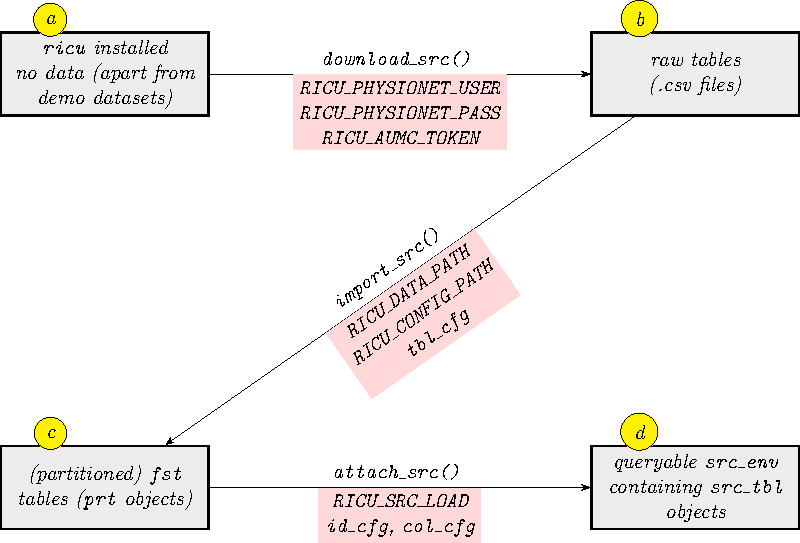
\includegraphics{/private/var/folders/24/8k48jl6d249_n_qfxwsl6xvm0000gn/T/RtmphhAogK/file14632599b224/articles/jss_files/figure-latex/src-setup-1} 

}

\caption[Making a dataset available to \pkg{ricu} involves several steps, starting with data download, followed by preparation for efficient access and finalized by instantiation of data structures containing relevant metadata]{Making a dataset available to \pkg{ricu} involves several steps, starting with data download, followed by preparation for efficient access and finalized by instantiation of data structures containing relevant metadata. The functions which are used for each step are displayed above arrows and below (in red) are indicated specific configuration settings or environment variables which are need for (or can be used to customize) the specific step.}\label{fig:src-setup}
\end{figure}
\end{CodeChunk}

\hypertarget{data-download}{%
\subsubsection{Data download}\label{data-download}}

The first step towards accessing data is data download, taken care of by
the S3 generic function \texttt{download\_src()}. For the datasets
included with \pkg{ricu}, prior to calling \texttt{download\_src()}, the
following environment variables can be set (indicated in red in the
\(a \to b\) edge in Figure \ref{fig:src-setup}):

\begin{itemize}
\tightlist
\item
  \texttt{RICU\_PHYSIONET\_USER}/\texttt{RICU\_PHYSIONET\_PASS}:
  PhysioNet login credentials with access to the requested dataset(s).
\item
  \texttt{RICU\_AUMC\_TOKEN}: Download token, extracted from the
  download URL received after being granted data access.
\end{itemize}

If any of the required access credentials are not available as
environment variables, they can be supplied as function arguments to
\texttt{download\_src()} or the user is queried in interactive sessions
and an error is thrown otherwise.

As a quick reminder on system requirements for initial data setup
operations: Each of the supported datasets requires 5-10 GB disk space
for permanent storage and 50-100 GB of temporary disk storage during
download and import. Memory requirements are kept low (8-16 GB) by
performing all setup operations only on subsets of rows at the time.
Initial data source setup can be expected to take upwards of an hour per
dataset.

\hypertarget{data-import}{%
\subsubsection{Data import}\label{data-import}}

After successful data download, importing prepares tables for efficient
random row- and column-access, for which the raw data format (.csv) is
not well suited (see edge \(b \to c\) in Figure \ref{fig:src-setup}).
Tables are read in using \pkg{readr} \citep{hester2020}, potentially
(re-)partitioned row-wise, and re-saved using \pkg{fst}. Environment
variables that can be set to customize \pkg{ricu} data handling,
relevant for import and attaching include:

\begin{itemize}
\tightlist
\item
  \texttt{RICU\_DATA\_PATH}: Optional data storage location (if unset,
  this defaults to a system-specific, user-specific directory). The
  current value used for this setting can be queried by calling
  \texttt{data\_dir()}.
\item
  \texttt{RICU\_CONFIG\_PATH}: A comma-separated set of paths to
  directories containing configuration files. The current set of paths
  is retrievable by calling \texttt{config\_paths()} and the ordering of
  paths determines precedence of how configuration files are combined
  (if multiple files of the same name are available).
\end{itemize}

For importing, the information contained in \texttt{tbl\_cfg}
configuration objects is most relevant. This determines column data
types, table partitioning and sanity checks like number of rows per
table. Please refer to Section \ref{table-configuration} for more
information on the construction of \texttt{tbl\_cfg} objects.

\hypertarget{data-attaching}{%
\subsubsection{Data attaching}\label{data-attaching}}

Finally, attaching a dataset creates a corresponding \texttt{src\_env}
object, containing a corresponding \texttt{src\_tbl} object for each
table, which together with associated metadata are used by \pkg{ricu} to
run queries against the data (edge \(c \to d\) in Figure
\ref{fig:src-setup}). The environment variable \texttt{RICU\_SRC\_LOAD}
may contain a comma-separated list of data source names that are set up
for being automatically attached on namespace loading. This defaults to
all currently supported datasets and the active set of source names is
available as \texttt{auto\_attach\_srcs()}. Apart from this automatism,
the process of attaching a dataset can be manually invoked by calling
\texttt{attach\_src()}, which can be convenient when for example
updating the data source configuration after it has been modified.

Two configuration objects which are important for data loading (see the
following Section \ref{data-loading}) are \texttt{id\_cfg} and
\texttt{col\_cfg} (described in Sections \ref{id-configuration} and
\ref{default-column-configuration}, respectively), providing default
values for certain types of columns, including time-stamp, measurement
value and measurement unit column names, as well as defining
relationships between patient identifiers (such as hospital stay ID and
ICU stay ID).

\hypertarget{data-loading}{%
\subsection{Data loading}\label{data-loading}}

The lowest level of data access is direct subsetting of
\texttt{src\_tbl} objects as shown at the start of Section
\ref{data-sources}. As \texttt{src\_tbl} inherits from \texttt{prt}, the
\texttt{subset()} implementation provided by \pkg{prt} can be used for
NSE of data-expressions against on-disk, tabular data. Building on that,
several S3 generic functions successively homogenize data
representations as visualized in Figure \ref{fig:data-loading}.

\begin{CodeChunk}
\begin{figure}

{\centering 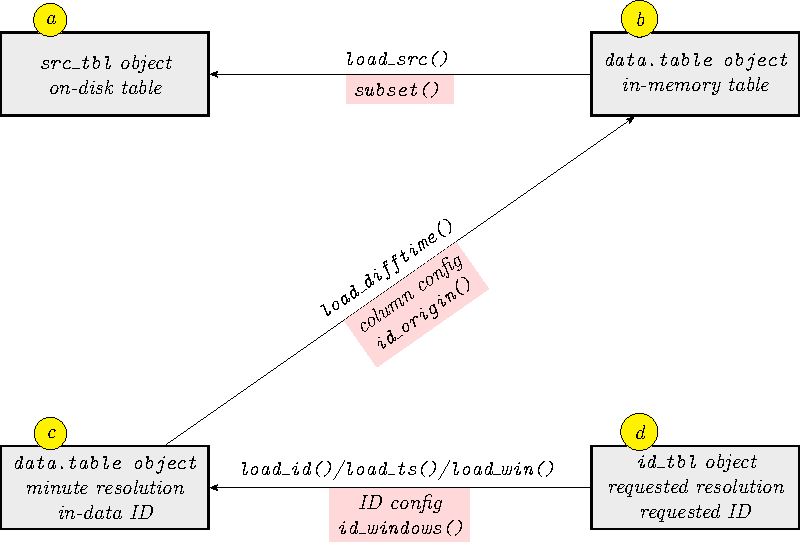
\includegraphics{/private/var/folders/24/8k48jl6d249_n_qfxwsl6xvm0000gn/T/RtmphhAogK/file14632599b224/articles/jss_files/figure-latex/data-loading-1} 

}

\caption{Data loading proceeds through several layers, each contributing a step towards harmonizing discrepancies among raw data representations provided by the different data sources. Raw data tables are represented by \pkg{ricu} as \code{src\_tbl} objects which can be queried using \code{load\_src()}. Absolute time-stamps in the returned \code{data.table} are converted to times relative to admission (in minutes) by \code{load\_difftime()} and finally, \code{load\_id()}/\allowbreak\code{load\_ts()}/\allowbreak\code{load\_win()} ensure a given ID system and time interval.}\label{fig:data-loading}
\end{figure}
\end{CodeChunk}

The most basic layer in data loading is provided by the S3 generic
function \texttt{load\_src()}, which provides a string-based interface
to the \texttt{cols} argument of \texttt{subset()} while forwarding the
unevaluated expression passed as \texttt{rows} (see edge \(a \to b\) in
Figure \ref{fig:data-loading}).

\begin{CodeChunk}
\begin{CodeInput}
R> load_src(mimic_demo$admissions, subject_id > 44000,
+          cols = c("hadm_id", "admittime", "dischtime"))
\end{CodeInput}
\begin{CodeOutput}
   hadm_id           admittime           dischtime
1:  125157 2112-05-04 08:00:00 2112-05-11 14:15:00
2:  131048 2112-05-22 15:37:00 2112-05-25 13:30:00
3:  198330 2112-05-28 15:45:00 2112-06-07 16:50:00
4:  174245 2178-05-14 20:29:00 2178-05-15 09:45:00
5:  163189 2123-11-24 14:14:00 2123-12-30 14:31:00
6:  192189 2180-07-19 06:55:00 2180-07-20 13:00:00
7:  103379 2170-12-15 03:14:00 2170-12-24 18:00:00
\end{CodeOutput}
\end{CodeChunk}

As data sources differ in their representation of time-stamps, a next
step in data homogenization is to converge to a common format: the time
difference to the origin time-point of a given ID system (for example
ICU admission).

\begin{CodeChunk}
\begin{CodeInput}
R> load_difftime(mimic_demo$admissions, subject_id > 44000,
+               cols = c("hadm_id", "admittime", "dischtime"))
\end{CodeInput}
\end{CodeChunk}

\begin{CodeChunk}
\begin{CodeOutput}
# An `id_tbl`: 7 x 3
# Id var:      `hadm_id`
  hadm_id admittime dischtime
    <int> <drtn>    <drtn>
1  103379 0 mins    13846 mins
2  125157 0 mins    10455 mins
3  131048 0 mins     4193 mins
4  163189 0 mins    51857 mins
5  174245 0 mins      796 mins
6  192189 0 mins     1805 mins
7  198330 0 mins    14465 mins
\end{CodeOutput}
\end{CodeChunk}

The function \texttt{load\_difftime()} is expected to return timestamps
as base \proglang{R} \texttt{difftime} vectors (in minutes; edge
\(b \to c\) in Figure \ref{fig:data-loading}). The argument
\texttt{id\_hint} can be used to specify a preferred ID system, but if
not available in raw data, \texttt{load\_difftime()} will return data
using the ID system with highest cardinality (i.e., ICU stay ID is
preferred over hospital stay ID). In the above example, if
\texttt{icustay\_id} were requested, data would be returned using
\texttt{hadm\_id}, whereas a \texttt{subject\_id} request would be
honored, as the corresponding ID column is available in the
\texttt{admissions} table.

Building on \texttt{load\_difftime()} functionality, functions
\texttt{load\_id()}/\allowbreak\texttt{load\_ts()}/\allowbreak\texttt{load\_win()}
return
\texttt{id\_tbl}/\allowbreak\texttt{ts\_tbl}/\allowbreak\texttt{win\_tbl}
objects with the requested ID system (passed as \texttt{id\_var}
argument). This uses raw data IDs if available or calls
\texttt{change\_id()} in order to convert to the desired ID system (edge
\(c \to d\) in Figure \ref{fig:data-loading}). Similarly, where
\texttt{load\_difftime()} returns data with fixed time interval of one
minute, \texttt{load\_id()} allows for arbitrary time intervals (using
\texttt{change\_interval()}; defaults to 1 hour).

\begin{CodeChunk}
\begin{CodeInput}
R> load_id(mimic_demo$admissions, subject_id > 44000,
+         cols = c("admittime", "dischtime"), id_var = "hadm_id")
\end{CodeInput}
\end{CodeChunk}

\begin{CodeChunk}
\begin{CodeOutput}
# An `id_tbl`: 7 x 3
# Id var:      `hadm_id`
  hadm_id admittime dischtime
    <int> <drtn>    <drtn>
1  103379 0 hours   230 hours
2  125157 0 hours   174 hours
3  131048 0 hours    69 hours
4  163189 0 hours   864 hours
5  174245 0 hours    13 hours
6  192189 0 hours    30 hours
7  198330 0 hours   241 hours
\end{CodeOutput}
\end{CodeChunk}

Throughout several of theses functions, \texttt{col\_cfg} objects are
used to provide sensible defaults. In order to convert to relative
times, \texttt{load\_difftime()}, for example, requires names of columns
for which this applies (provided by the \texttt{time\_vars} entry), and
\texttt{load\_ts()} needs to know which of the \texttt{time\_vars} to
use as \texttt{index\_var}. For more information on the construction of
\texttt{col\_cfg} objects, please refer to Section
\ref{default-column-configuration}.

A call to \texttt{change\_id()} requires the construction of a table
which contains the mapping between different ID systems, together with
information about how to convert timestamps between these ID systems
(edge \(c \to d\) in Figure \ref{fig:data-loading}). The function
responsible for providing the necessary information is
\texttt{id\_windows()} and the associated S3 generic function
\texttt{id\_win\_helper()}. The entry point \texttt{id\_windows()} wraps
\texttt{id\_win\_helper()}, providing memoization, as the resulting
structure is expensive to compute relative to the frequency of being
required.

\begin{CodeChunk}
\begin{CodeInput}
R> id_windows(mimic_demo)
\end{CodeInput}
\begin{CodeOutput}
# An `id_tbl`: 136 x 9
# Id var:      `icustay_id`
    icustay_id hadm_id subject_id icustay_id_start hadm_id_start
         <int>   <int>      <int> <drtn>           <drtn>
  1     201006  198503      10076 0 mins            -3290 mins
  2     201204  114648      42321 0 mins               -2 mins
  3     203766  126949      10045 0 mins            -1336 mins
  4     204132  157609      40310 0 mins               -1 mins
  5     204201  177678      10104 0 mins             -368 mins
...
132     295043  170883      10124 0 mins           -10413 mins
133     295741  176805      10090 0 mins               -1 mins
134     296804  110244      10035 0 mins            -1294 mins
135     297782  167612      43909 0 mins               -1 mins
136     298685  151323      42075 0 mins               -1 mins
# ... with 126 more rows, and 4 more variables: subject_id_start <drtn>,
#   icustay_id_end <drtn>, hadm_id_end <drtn>, subject_id_end <drtn>
\end{CodeOutput}
\end{CodeChunk}

Analogously, the function pair \texttt{id\_origin()} and
\texttt{id\_orig\_helper()}, with the former wrapping the latter and
again providing memoization, is used for datasets where time-stamps are
represented by absolute times, returning the origin time-points for a
given ID system which then can be used to calculate relative times (edge
\(b \to c\) in Figure \ref{fig:data-loading}).

\begin{CodeChunk}
\begin{CodeInput}
R> id_origin(mimic_demo, "icustay_id")
\end{CodeInput}
\begin{CodeOutput}
# An `id_tbl`: 136 x 2
# Id var:      `icustay_id`
    icustay_id intime
         <int> <dttm>
  1     201006 2107-03-24 04:06:14
  2     201204 2121-12-07 20:50:36
  3     203766 2129-11-24 22:46:57
  4     204132 2144-12-24 16:16:41
  5     204201 2120-08-24 23:47:23
...
132     295043 2192-04-24 02:29:49
133     295741 2124-01-12 14:27:16
134     296804 2129-03-04 13:40:11
135     297782 2152-10-09 19:05:36
136     298685 2166-02-12 17:57:37
# ... with 126 more rows
\end{CodeOutput}
\end{CodeChunk}

For the included datasets, the implementations of
\texttt{id\_win\_helper()} and \texttt{id\_orig\_helper()}, use
information contained in \texttt{id\_cfg} objects (see Section
\ref{id-configuration}) to determine which columns in which tables are
required for constructing the corresponding lookup tables. Doing so,
however, is not necessary: an \texttt{id\_win\_helper()} implementation
for a new dataset could forego this by hard-coding table/column names as
part of the function logic, in-turn simplifying the corresponding
\texttt{id\_cfg} object to merely providing naming and ordering
information.

\hypertarget{data-source-configuration}{%
\subsection{Data source configuration}\label{data-source-configuration}}

Data source environments (and corresponding \texttt{src\_tbl} objects)
are constructed using source configuration objects: list-based
structures, inheriting from \texttt{src\_cfg} and from any number of
data source specific class names with suffix \texttt{\_cfg} appended (as
discussed at the beginning of Section \ref{data-sources}). The exported
function \texttt{load\_src\_cfg()} reads a JSON formatted file and
creates a \texttt{src\_cfg} object per data source and further therein
contained objects.

\begin{CodeChunk}
\begin{CodeInput}
R> cfg <- load_src_cfg("mimic_demo")
R> str(cfg, max.level = 3L, width = 70L)
\end{CodeInput}
\begin{CodeOutput}
List of 1
 $ mimic_demo:List of 6
  ..$ name   : chr "mimic_demo"
  ..$ prefix : chr [1:2] "mimic_demo" "mimic"
  ..$ id_cfg : id_cfg [1:3] `subject_id`, `hadm_id`, `icustay_id`
  ..$ col_cfg: col_cfg [1:25] [0, 0, 5, 0, 1], [0, 1, 6, 0, 1], [1, 0, 0...
  ..$ tbl_cfg: tbl_cfg [1:25] [?? x 19; 1], [?? x 24; 1], [?? x 4; 1], [...
  ..$ extra  :List of 1
  .. ..$ url: chr "https://physionet.org/files/mimiciii-demo/1.4"
  ..- attr(*, "class")= chr [1:3] "mimic_demo_cfg" "mimic_cfg" "src_cfg"
\end{CodeOutput}
\begin{CodeInput}
R> mi_cfg <- cfg[["mimic_demo"]]
\end{CodeInput}
\end{CodeChunk}

In addition to required fields \texttt{name} and \texttt{prefix} (used
as class prefix), as well as further arbitrary fields contained in
\texttt{extra} (\texttt{url} in this case), several configuration
objects are part of \texttt{src\_cfg}: \texttt{id\_cfg},
\texttt{col\_cfg} and \texttt{tbl\_cfg}.

\hypertarget{id-configuration}{%
\subsubsection{ID configuration}\label{id-configuration}}

An \texttt{id\_cfg} object contains an ordered set of key-value pairs
representing patient identifiers in a dataset. An implicit assumption
currently is that a given patient ID system is used consistently
throughout a dataset, meaning that for example an ICU stay ID is always
referred to by the same name throughout all tables containing a
corresponding column. Owing to the relational origins of these datasets
this has been fulfilled in all instances encountered so far. In
MIMIC-III, ID systems

\begin{CodeChunk}
\begin{CodeInput}
R> as_id_cfg(mi_cfg)
\end{CodeInput}
\begin{CodeOutput}
<id_cfg<mimic_demo[patient < hadm < icustay]>[3]>
     patient         hadm      icustay 
`subject_id`    `hadm_id` `icustay_id` 
\end{CodeOutput}
\end{CodeChunk}

are available, allowing for identification of individual patients, their
(potentially multiple) hospital admissions over the course of the years
and their corresponding ICU admissions (as well as potential
re-admissions). Ordering corresponds to cardinality: moving to larger
values implies moving along a one-to-many relationship. This information
is used in data-loading, whenever the target ID system is not contained
in the raw data.

\hypertarget{default-column-configuration}{%
\subsubsection{Default column
configuration}\label{default-column-configuration}}

Again used in data loading, this per-table set of key-value pairs
specifies column defaults as \texttt{col\_cfg} object. Each key
describes a type of column with special meaning and the corresponding
value specifies said column for a given table. The print method for
\texttt{col\_cfg} reports all keys alongside the per-table counts of
accordingly registered values (i.e., columns).

\begin{CodeChunk}
\begin{CodeInput}
R> as_col_cfg(mi_cfg)
\end{CodeInput}
\begin{CodeOutput}
<col_cfg<mimic_demo[id_var, index_var, time_vars, unit_var, val_var]>[25]>
        admissions            callout         caregivers        chartevents 
   [0, 0, 5, 0, 1]    [0, 1, 6, 0, 1]    [1, 0, 0, 0, 1]    [0, 1, 2, 1, 1] 
         cptevents              d_cpt    d_icd_diagnoses   d_icd_procedures 
   [0, 1, 1, 0, 1]    [1, 0, 0, 0, 1]    [1, 0, 0, 0, 1]    [1, 0, 0, 0, 1] 
           d_items         d_labitems     datetimeevents      diagnoses_icd 
   [1, 0, 0, 0, 1]    [1, 0, 0, 0, 1]    [0, 1, 3, 0, 1]    [0, 0, 0, 0, 1] 
          drgcodes           icustays     inputevents_cv     inputevents_mv 
   [0, 0, 0, 0, 1]    [0, 1, 2, 0, 1]    [0, 1, 2, 1, 1]    [0, 1, 4, 1, 1] 
         labevents microbiologyevents       outputevents           patients 
   [0, 1, 1, 1, 1]    [0, 1, 2, 0, 1]    [0, 1, 2, 1, 1]    [0, 0, 4, 0, 1] 
     prescriptions procedureevents_mv     procedures_icd           services 
   [0, 1, 2, 1, 1]    [0, 1, 4, 1, 1]    [0, 0, 0, 0, 1]    [0, 1, 1, 0, 1] 
         transfers 
   [0, 1, 2, 0, 1] 
\end{CodeOutput}
\end{CodeChunk}

The following column defaults are currently in use throughout \pkg{ricu}
but the set of keys can be extended to arbitrary new values:

\begin{itemize}
\tightlist
\item
  \texttt{id\_var}: In case a table does not contain at least one ID
  column corresponding to one of the ID systems specified as
  \texttt{id\_cfg}, the default ID column can be set on a per-table
  basis as \texttt{id\_var}\footnote{This for example is the case for
    the \texttt{d\_items} table in MIMIC-III, which does not contain any
    patient related data, but holds information on items encoding types
    of measurements, procedures, etc., used throughout other tables
    holding actual patient data.}.
\item
  \texttt{index\_var}: A column that is used to define an ordering in
  time over rows, thereby providing a time series index\footnote{For the
    MIMIC-III table \texttt{inputevents\_mv}, of the four available time
    variables (\texttt{starttime}, \texttt{endtime}, \texttt{storetime},
    \texttt{comments\_date}), \texttt{starttime} lends itself to be used
    as index variable more than the other candidates and therefore is
    set as default.}.
\item
  \texttt{time\_vars}: Columns which will be treated as time variables
  (important for converting between ID systems for example), but not as
  time series indices\footnote{In case of the \texttt{admissions} table
    in MIMIC-III for example, a total of five columns are considered to
    be time variables, none of which stands out as potential
    \texttt{index\_var}.}.
\item
  \texttt{unit\_var}: Used in concept loading (more specifically for
  \texttt{num\_cncpt} concepts, see Section \ref{concept-specification})
  to identify columns that represent unit of measurement information.
\item
  \texttt{val\_var}: Again used when loading data concepts, this
  identified a default value variable in a table, representing the
  column of interest to be used as returned data column.
\end{itemize}

While \texttt{id\_var}, \texttt{index\_var} and \texttt{time\_vars} are
used to provide sensible defaults to functions used for general data
loading (Section \ref{data-loading}), \texttt{unit\_var},
\texttt{val\_var}, as well as potential user-defined defaults are only
used in concept loading (see Section \ref{ready-to-use-concepts}) and
therefore need not be prioritized when integrating new data sources
until data concepts have been mapped.

\hypertarget{table-configuration}{%
\subsubsection{Table configuration}\label{table-configuration}}

Finally, \texttt{tbl\_cfg} objects are used during the initial setup of
a data source. In order to create a representation of a table that is
accessible by \pkg{ricu} from raw data, several key pieces of
information are required:

\begin{itemize}
\item
  File name(s): In the simplest case, a single file corresponds to a
  single table. Other scenarios that have been encountered (and are
  therefore handled) include tables partitioned into multiple files and
  .tar archives containing multiple tables.
\item
  Column specification: For each column, the expected data type has to
  be known, as well as a pair of names, one corresponding to the raw
  data column name and one corresponding to the column name to be used
  within \pkg{ricu}.
\item
  (Optional) number of rows: Used as sanity check whenever available.
\item
  (Optional) partitioning information: For very \emph{long} tables it
  can be useful to specify a row-partitioning. This currently is only
  possible by applying a vector of breakpoints to a single numeric
  column, thereby defining a grouping.
\end{itemize}

Table configuration objects are only used within the context of the
functions \texttt{download\_src()} and \texttt{import\_src()} and are
therefore not required if download and import are carried out manually.

\begin{CodeChunk}
\begin{CodeInput}
R> as_tbl_cfg(mi_cfg)
\end{CodeInput}
\begin{CodeOutput}
<tbl_cfg<mimic_demo[rows x cols; partitions]>[25]>
        admissions            callout         caregivers        chartevents 
      [?? x 19; 1]       [?? x 24; 1]        [?? x 4; 1]       [?? x 15; 2] 
         cptevents              d_cpt    d_icd_diagnoses   d_icd_procedures 
      [?? x 12; 1]        [?? x 9; 1]        [?? x 4; 1]        [?? x 4; 1] 
           d_items         d_labitems     datetimeevents      diagnoses_icd 
      [?? x 10; 1]        [?? x 6; 1]       [?? x 14; 1]        [?? x 5; 1] 
          drgcodes           icustays     inputevents_cv     inputevents_mv 
       [?? x 8; 1]       [?? x 12; 1]       [?? x 22; 1]       [?? x 31; 1] 
         labevents microbiologyevents       outputevents           patients 
       [?? x 9; 1]       [?? x 16; 1]       [?? x 13; 1]        [?? x 8; 1] 
     prescriptions procedureevents_mv     procedures_icd           services 
      [?? x 19; 1]       [?? x 25; 1]        [?? x 5; 1]        [?? x 6; 1] 
         transfers 
      [?? x 13; 1] 
\end{CodeOutput}
\end{CodeChunk}

For the \texttt{chartevents} table of the MIMIC-III demo dataset, rows
are partitioned into two groups, while all other tables are represented
by a single partition. Furthermore, the expected number of rows is
unknown (\texttt{??}) as this is missing from the corresponding
\texttt{tbl\_cfg} object.

\hypertarget{adding-external-datasets}{%
\subsection{Adding external datasets}\label{adding-external-datasets}}

In order to add a new dataset to \pkg{ricu}, several aspects outlined in
the previous subsections require consideration. For illustration
purposes, code for integrating AmsterdamUMCdb as external dataset is
available from \href{https://github.com/eth-mds/aumc}{GitHub}. While
this is no longer needed for using the \texttt{aumc} data source, the
repository will remain as it might serve as template to integration of
new datasets. Throughout this repository (and the following paragraphs),
the AmsterdamUMCdb data treated as an \pkg{ricu}-external dataset is
referred to as \texttt{aumc\_ext}.

\hypertarget{adding-configuration-information}{%
\subsubsection{Adding configuration
information}\label{adding-configuration-information}}

Central to adding a new dataset to \pkg{ricu} is providing some
configuration information in a \texttt{data-sources.json} file pointed
to by the environment variable \texttt{RICU\_CONFIG\_PATH}. Depending on
particularities of the dataset in question, corresponding
implementations of some of the S3 generic functions mentioned throughout
Sections \ref{data-source-setup} and \ref{data-loading} might have to be
provided. The amount of confirmation information required to get started
also depends on the desired level of integration. As data download and
import are one-time procedures, these steps can be carried out manually,
negating the need for specifying column data types in
\texttt{data-sources.json} and providing data source specific methods
for the \texttt{download\_src()} and \texttt{import\_src()} generics.

The basic organization of a data source configuration entry, as it could
be used for \texttt{aumc\_ext}, specified as JSON is as follows:

\begin{verbatim}
{
  "name": "aumc_ext",
  "id_cfg": {
    "patient": {
      "id": "patientid",
      "position": 1
    },
    "icustay": {
      "id": "admissionid",
      "position": 2
    }
  },
  "tables": {
    ...
  }
}
\end{verbatim}

The shown \texttt{id\_cfg} entry represents the minimally required set
of entries, where for each ID specification, \texttt{start},
\texttt{end} and \texttt{table} are omitted (when compared to the
\texttt{aumc} configuration provided by \pkg{ricu}). The \texttt{tables}
entry expands to something like the following:

\begin{verbatim}
"tables": {
  "freetextitems": {
  },
  "drugitems": {
    "defaults": {
      "index_var": "start",
      "val_var": "dose",
      "unit_var": "doseunit",
      "time_vars": ["start", "stop"]
    }
  },
  "numericitems": {
    "defaults": {
      "index_var": "measuredat",
      "val_var": "value",
      "unit_var": "unit",
      "time_vars": ["measuredat", "registeredat", "updatedat"]
    },
    "partitioning": {
      "col": "",
      "breaks": [
        0, 0, 0, 0, 0, 0, 0, 0, 0, 0, 0, 0, 0, 0, 0, 0, 0, 0,
        0, 0, 0, 0, 0
      ]
    }
  },
  ...
}
\end{verbatim}

Minimally required is simply an entry indicating the data source
membership of a table (if not partitioned; cf., \texttt{freetextitems}).
This does slightly complicate data exploration, as if no
\texttt{defaults} are available, no default values can be provided to
calls to \texttt{load\_ts()} and related functions and therefore
repeatedly have to be specified in corresponding function calls. Also,
when specifying data items in such a setup, the per-table column names
for special columns such as \texttt{index\_var}, \texttt{val\_var},
etc., have to be repeated for each individual item entry.

For partitioned tables, the basic structure of a \texttt{partitioning}
entry is required, but the content itself is irrelevant, as this is only
used for setup (cf., \texttt{numericitems}). The length of
\texttt{breaks}, however, is required to match the number of partitions
(i.e., a length 23 \texttt{breaks} specification corresponds to a
partitioning into 24 row-groups.)\footnote{Originally it was intended to
  use partitioning information during data loading in order to narrow
  down the set of partitions that have to be accessed. So far, this
  optimization has not been implemented.}. The directory containing such
a \texttt{data-sources.json} can then be pointed to by the environment
variable \texttt{RICU\_CONFIG\_PATH}, making it available to \pkg{ricu}.

\hypertarget{enabling-data-loading}{%
\subsubsection{Enabling data loading}\label{enabling-data-loading}}

As for functions that are required, currently there is no default method
available for the loading step provided by \texttt{load\_difftime()} and
most likely an implementation of the generic function
\texttt{id\_win\_helper()} will be required as well. For
\texttt{aumc\_ext}, \texttt{load\_difftime()} could be implemented as

\begin{CodeChunk}
\begin{CodeInput}
R> ms_as_min <- function(x) {
+   as.difftime(as.integer(x / 6e4), units = "mins")
+ }
R> 
R> aumc_difftime <- function(x, rows, cols = colnames(x),
+                           id_hint = id_vars(x),
+                           time_vars = ricu::time_vars(x), ...) {
+ 
+   if (id_hint %in% colnames(x)) {
+     id_sel <- id_hint
+   } else {
+     id_opt <- id_var_opts(sort(as_id_cfg(x), decreasing = TRUE))
+     id_sel <- intersect(id_opt, colnames(x))[1L]
+   }
+ 
+   stopifnot(is.character(id_sel), length(id_sel) == 1L)
+ 
+   if (!id_sel %in% cols) {
+     cols <- c(id_sel, cols)
+   }
+ 
+   time_vars <- intersect(time_vars, cols)
+ 
+   dat <- load_src(x, {{ rows }}, cols)
+   dat <- dat[, c(time_vars) := lapply(.SD, ms_as_min),
+              .SDcols = time_vars]
+ 
+   as_id_tbl(dat, id_vars = id_sel, by_ref = TRUE)
+ }
\end{CodeInput}
\end{CodeChunk}

Such a function attempts to use the ID as requested as
\texttt{id\_hint}, but falls back to the best possible alternative
(using the ordering as previously specified in the \texttt{id\_cfg} JSON
configuration) if not provided by the data. The helper function
\texttt{id\_var\_opts()} returns the dataset-specific column names of an
\texttt{id\_cfg} object (as opposed to the dataset-agnostic ID names;
cf., \texttt{subject\_id} and \texttt{patient}). Both the row-subsetting
expression and column selection are passed on to \texttt{load\_src()}
and all columns specified as \texttt{time\_vars} are converted to
\texttt{difftime} vectors in minutes. Operations can safely be carried
out using by-reference semantics, as intermediate objects are not
exposed to the user.

For a possible implementation of the \texttt{id\_win\_helper()} generic,
column and table names to assemble the desired lookup table are hard
coded instead of provided by the corresponding \texttt{id\_cfg} object
(as is the case in the \pkg{ricu}-internal implementation).

\begin{CodeChunk}
\begin{CodeInput}
R> aumc_windows <- function(x) {
+ 
+   ids <- c("admissionid", "patientid")
+   sta <- c("admittedat", "firstadmittedat")
+   end <- c("dischargedat", "dateofdeath")
+ 
+   tbl <- as_src_tbl(x, "admissions")
+ 
+   res <- tbl[, c(ids, sta[1L], end)]
+   res <- res[, c(sta[2L]) := 0L]
+   res <- res[, c(sta, end) := lapply(.SD, ms_as_min),
+              .SDcols = c(sta, end)]
+ 
+   res <- data.table::setcolorder(res, c(ids, sta, end))
+   res <- rename_cols(res, c(ids, paste0(ids, "_start"),
+                                  paste0(ids, "_end")), by_ref = TRUE)
+ 
+   as_id_tbl(res, ids[2L], by_ref = TRUE)
+ }
\end{CodeInput}
\end{CodeChunk}

As all the required information is available form the
\texttt{admissions} table, \texttt{aumc\_windows()} simply loads the
corresponding columns, converts them to minute resolution, followed by
some renaming. ICU admissions and discharges in this table are relative
to initial hospital admissions and therefore an all-zero column
\texttt{firstadmittedat} is added and the \texttt{id\_var} of the
resulting \texttt{id\_tbl} is marked as \texttt{patientid}\footnote{The
  patient ID created in this way is different to that available for
  MIMIC-III, where patient date of birth is provided. An approximate
  date of birth could be constructed if ages were reported more
  precisely, but given the rough binning available here, this might be
  considered an acceptable limitation of resulting patient IDs.
  Nevertheless awareness of such differences in data presentation is
  important.}.

A final step in making a new dataset accessible to \pkg{ricu} lies in
specifying concept items. To this end, a file \texttt{concept-dict.json}
can be added to the directory pointed to by the environment variable
\texttt{RICU\_CONFIG\_PATH}, containing entries like the following,
which will make it possible to use the \texttt{hr} concept across all
datasets included with \pkg{ricu}, alongside the newly added dataset.

\begin{verbatim}
{
  "hr": {
    "sources": {
      "aumc_ext": [
        {
          "ids": 6640,
          "table": "numericitems",
          "sub_var": "itemid"
        }
      ]
    }
  }
}
\end{verbatim}

The above outline serves as an example on how to proceed when adding new
data to \pkg{ricu}. Aspects like having multiple patient IDs, for
example, could be further simplified\footnote{An example for such a
  reduced setup is available from the
  \href{https://github.com/eth-mds/aumc}{AUMC GitHub repository} as
  \texttt{aumc\_min}. Moving to only a single patient identifier also
  does away with the need for a \texttt{id\_win\_helper()}
  implementation, as \texttt{change\_id()} will not be called in such a
  scenario.}. Owing to the extensive use of S3 generic functions,
\pkg{ricu} offers considerable flexibility for customizing certain
behavior to specifics of a given data source, while providing fallback
procedures whenever more general treatment can be applied.

\hypertarget{summary-of-required-steps}{%
\subsubsection{Summary of required
steps}\label{summary-of-required-steps}}

Summarizing aspects explained in more detail in the previous sections,
the following points list the required steps for adding new data in the
order they should be considered in. The approach taken here being is to
start simple and expand.

\begin{enumerate}
\def\labelenumi{\arabic{enumi}.}
\item
  Tables saved as \texttt{.fst} files should be moved to the folder
  returned by \texttt{src\_data\_dir()} when passed the dataset name
  (alternatively, methods implementing \texttt{src\_download()} and
  \texttt{src\_import()} are required).
\item
  A minimal data source configuration file \texttt{data-sources.json} is
  required in the directory pointed to by \texttt{RICU\_CONFIG\_PATH}.
  For AmsterdamUMCdb, this could be as minimal as (assuming no
  partitioning):

\begin{verbatim}
 {
   "name": "aumc_min",
   "id_cfg": {
     "icustay": "admissionid"
   },
   "tables": {
     "admissions": {},
     "drugitems": {},
     "freetextitems": {},
     "listitems": {},
     "numericitems": {},
     "procedureorderitems": {},
     "processitems": {}
   }
 }
\end{verbatim}

  File names have to match table names, i.e., the admissions table
  should be named \texttt{admissions.fst}. Upon a call to
  \texttt{attach\_src()} (or next loading of the package and having
  added the data source name to \texttt{RICU\_SRC\_LOAD}) the new data
  source can be explored using \texttt{load\_src()}.
\item
  A \texttt{load\_difftime()} method is required, which:

  \begin{itemize}
  \tightlist
  \item
    passes a row-subsetting expression to \texttt{load\_src()} using the
    \pkg{rlang} curly-curly operator,
  \item
    converts columns passed as \texttt{time\_vars} to minute-resolution
    \texttt{difftime} vectors,
  \item
    returns an \texttt{id\_tbl} object where patient identifiers are
    chosen such that time-stamps are relative to corresponding
    admission,
  \item
    (optionally) uses the column passed as \texttt{id\_hint} for patient
    identifiers, if multiple identifiers are available from data.
  \end{itemize}

  Upon registering this method with S3 dispatch, higher-level data
  loading functions such as \texttt{load\_ts()} become available (given
  that no changes in patient identifiers are requested).
\item
  (Optional) if the source configuration specifies multiple patient
  identifiers which are not all available from all tables directly, an
  implementation of \texttt{id\_win\_helper()} most likely will be
  required (see Section \ref{data-loading}).
\item
  Now, the source configuration can be expanded with per-table column
  defaults and data items can be added to the concepts included with
  \pkg{ricu} by creating a \texttt{concept-dict.json} under the path
  pointed to by \texttt{RICU\_CONFIG\_PATH}. For more information on
  readily available concepts, refer to Section
  \ref{ready-to-use-concepts} and for specifying new concepts
  altogether, pointers are available in section
  \ref{concept-specification}.
\end{enumerate}

\hypertarget{examples}{%
\section{Examples}\label{examples}}

In order to briefly illustrate how \pkg{ricu} could be applied to
real-world clinical questions, two examples are provided in the
following sections. The first example fully relies on data concepts that
are included with \pkg{ricu}. Whereas the second one explores both how
some data preprocessing can be added to an existing concept, by creating
a recursive concept (or \texttt{rec\_cncpt}), as well as how to create
an entirely new data concept in code (instead of JSON specification as
outlined in Section \ref{concept-specification}), using constructors
\texttt{item()} and \texttt{concept()}.

\hypertarget{lactate-and-mortality}{%
\subsection{Lactate and mortality}\label{lactate-and-mortality}}

First, the association of lactate levels and mortality is investigated.
This problem has been studied before and it is widely accepted that both
static and dynamic lactate indices are associated with increased
mortality \citep{haas2016, nichol2011, van2013}. In order to model this
relationship, a time-varying proportional hazards Cox model
\citep{therneau2000, therneau2015} is fitted, which includes the SOFA
score as a general predictor of illness severity, using MIMIC-III demo
data. Furthermore, for the sake of this example, the patient cohort is
defined to be patients admitted from 2008 onwards (corresponding to the
MetaVision database) of ages 20 to 90 years old.

\begin{CodeChunk}
\begin{CodeInput}
R> src <- "mimic_demo"
R> 
R> cohort <- load_id("icustays", src, dbsource == "metavision",
+                   cols = NULL)
R> cohort <- load_concepts("age", src, patient_ids = cohort,
+                         verbose = FALSE)
R> 
R> dat <- load_concepts(c("lact", "death", "sofa"), src,
+                      patient_ids = cohort[age > 20 & age < 90, ],
+                      verbose = FALSE)
R> 
R> dat <- dat[,
+   head(.SD, n = match(TRUE, death, .N)), by = c(id_vars(dat))
+ ]
R> 
R> dat <- fill_gaps(dat)
R> 
R> dat <- replace_na(dat, c(NA, FALSE), type = c("locf", "const"),
+                   by_ref = TRUE, vars = c("lact", "death"),
+                   by = id_vars(dat))
R> 
R> cox_mod <- coxph(
+   Surv(charttime - 1L, charttime, death) ~ lact + sofa,
+   data = dat
+ )
\end{CodeInput}
\end{CodeChunk}

After loading the data, some minor preprocessing is still required
before modeling: first, data is filtered such that only data up to (and
including) the hour in which the \texttt{death} flag switches to
\texttt{TRUE} is used. Following that, missing values for \texttt{lact}
are imputed using a last observation carry forward (LOCF) scheme
(observing the patient grouping) and missing \texttt{death} values are
set to \texttt{FALSE}. The resulting model fit can be visualized as:

\begin{CodeChunk}


\begin{center}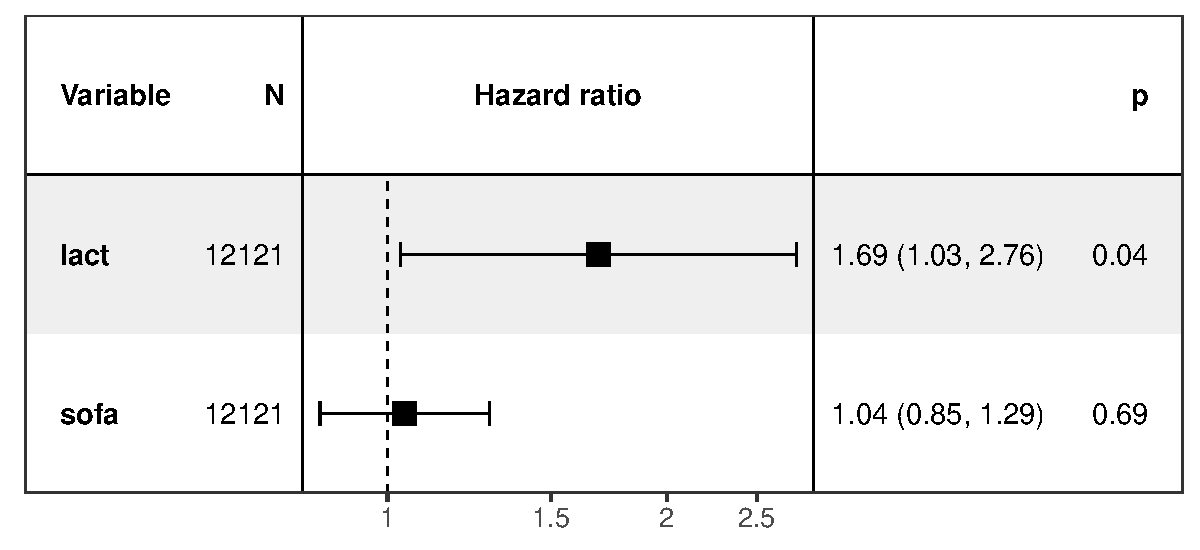
\includegraphics{/private/var/folders/24/8k48jl6d249_n_qfxwsl6xvm0000gn/T/RtmphhAogK/file14632599b224/articles/jss_files/figure-latex/cox-plot-1} \end{center}

\end{CodeChunk}

A simple exploration already shows that the increased values of lactate
are associated with mortality, even after adjusting for the SOFA score.
Using abstractions provided by \pkg{ricu}, this analysis could now also
be applied to other datasets with minimal effort.

\hypertarget{diabetes-and-insulin-treatment}{%
\subsection{Diabetes and insulin
treatment}\label{diabetes-and-insulin-treatment}}

For the next example, again using MIMIC-III demo data, comorbidities and
treatment related information are used: the amount of insulin
administered to patients in the first 24 hours from their ICU admission
is analyzed, in connection with diabetic status, in order to determine
whether diabetic patients receive more insulin over that time-span, when
compared to non-diabetic patients. For this, two concepts are
introduced: \texttt{ins24}, a binned variable representing the
cumulative amount of insulin administered within the first 24 hours of
an ICU admission, and \texttt{diab}, a logical variable encoding
diabetes comorbidity.

As there already is an insulin concept available, \texttt{ins24} can be
implemented as \texttt{rec\_cncpt}, requesting data from the
\texttt{ins} concept. In order to be able to calculate the total amount
of insulin administered, it is required to change the default
aggregation method from \texttt{median()} to \texttt{sum()}. Failing to
do so would yield under-reported values whenever several insulin
administrations fall within a given time-step. The callback function
\texttt{ins\_cb()} is then inserted into the loading process, performing
of the preprocessing steps outlined above: first data is subsetted to
fall into the first 24 hours of ICU admissions, followed by binning of
summed values.

\begin{CodeChunk}
\begin{CodeInput}
R> ins_breaks <- c(0, 1, 10, 20, 40, Inf)
R> 
R> ins_cb <- function(ins, ...) {
+ 
+   day_one <- function(x) x >= hours(0L) & x <= hours(24L)
+ 
+   idx_var <- index_var(ins)
+   ids_var <- id_vars(ins)
+ 
+   ins <- ins[
+     day_one(get(idx_var)), list(ins24 = sum(ins)), by = c(ids_var)
+   ]
+ 
+   ins <- ins[,
+     ins24 := list(cut(ins24, breaks = ins_breaks, right = FALSE))
+   ]
+ 
+   ins
+ }
R> 
R> ins24 <- load_dictionary(src, "ins")
R> ins24 <- concept("ins24", ins24, "insulin in first 24h",
+                  aggregate = "sum", callback = ins_cb,
+                  target = "id_tbl", class = "rec_cncpt")
\end{CodeInput}
\end{CodeChunk}

The binary diabetes concept can be implemented as \texttt{lgl\_cncpt},
for which ICD-9 codes are matched using a regular expression. As not
only the subset of diabetic patients is of interest, a \texttt{col\_itm}
is more suited for diabetes status retrieval over a \texttt{rgx\_itm}.
For creating the required callback function, which produces a logical
vector, the exported function factory \texttt{transform\_fun()} can be
employed, coupled with a function like \texttt{grep\_diab()}, performing
the desired transformation. The two concepts are then combined using
\texttt{c()} and loaded via \texttt{load\_concepts()}.

\begin{CodeChunk}
\begin{CodeInput}
R> grep_diab <- function(x) {
+   grepl("^250\\.?[0-9]{2}$", x)
+ }
R> 
R> diab  <- item(src, table = "diagnoses_icd",
+               callback = transform_fun(grep_diab),
+               class = "col_itm")
R> 
R> diab  <- concept("diab", diab, "diabetes", target = "id_tbl",
+                  class = "lgl_cncpt")
R> 
R> dat <- load_concepts(c(ins24, diab), id_type = "icustay",
+                      verbose = FALSE)
R> dat <- replace_na(dat, "[0,1)", vars = "ins24")
R> 
R> dat
\end{CodeInput}
\end{CodeChunk}

Following this, the difference between the two groups can be visualized
with a histogram over the binned insulin administration values:

\begin{CodeChunk}


\begin{center}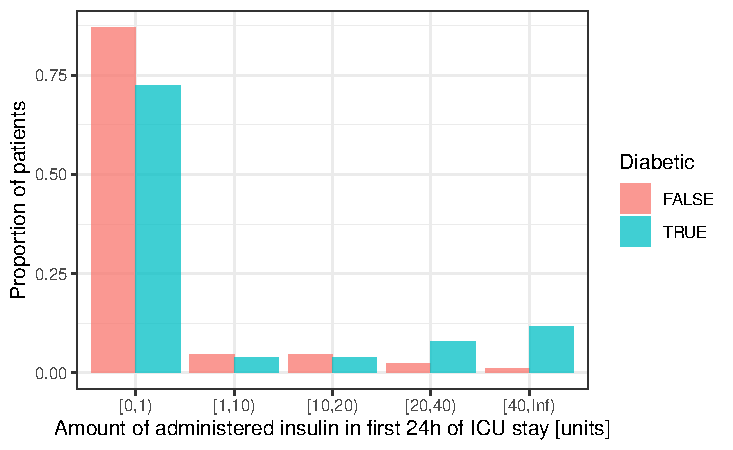
\includegraphics{/private/var/folders/24/8k48jl6d249_n_qfxwsl6xvm0000gn/T/RtmphhAogK/file14632599b224/articles/jss_files/figure-latex/diabetes-visualize-1} \end{center}

\end{CodeChunk}

The plot suggests that for the MetaVision cohort defined in the previous
example (without age subsetting) and during the first day of ICU stay,
perhaps unsurprisingly, with increasing insulin dosage, diabetic
patients receive more insulin compared to non-diabetic patients. This
effect is more pronounced when looking at the full MIMIC-III data
instead of the demo subset which includes only data corresponding to
roughly 130 ICU stays.

\hypertarget{acknowledgments}{%
\section{Acknowledgments}\label{acknowledgments}}

Nicolas Bennett, Drago Plečko, Nicolai Meinshausen and Peter Bühlmann
were supported by grant \#2017-110 of the Strategic Focal Area
``Personalized Health and Related Technologies (PHRT)'' of the ETH
Domain for the SPHN/PHRT Driver Project ``Personalized Swiss Sepsis
Study''.

\bibliography{jss.bib}


\end{document}

